%%%%%%%%%%%%%%%%%%%%%%%%%%%%%%%%%%%%%%%%%
% The Legrand Orange Book
% LaTeX Template
% Version 2.1.1 (14/2/16)
%
% This template has been downloaded from:
% http://www.LaTeXTemplates.com
%
% Original author:
% Mathias Legrand (legrand.mathias@gmail.com) with modifications by:
% Vel (vel@latextemplates.com)
%
% License:
% CC BY-NC-SA 3.0 (http://creativecommons.org/licenses/by-nc-sa/3.0/)
%
% Compiling this template:
% This template uses biber for its bibliography and makeindex for its index.
% When you first open the template, compile it from the command line with the 
% commands below to make sure your LaTeX distribution is configured correctly:
%
% 1) pdflatex main
% 2) makeindex main.idx -s StyleInd.ist
% 3) biber main
% 4) pdflatex main x 2
%
% After this, when you wish to update the bibliography/index use the appropriate
% command above and make sure to compile with pdflatex several times 
% afterwards to propagate your changes to the document.
%
% This template also uses a number of packages which may need to be
% updated to the newest versions for the template to compile. It is strongly
% recommended you update your LaTeX distribution if you have any
% compilation errors.
%
% Important note:
% Chapter heading images should have a 2:1 width:height ratio,
% e.g. 920px width and 460px height.
%
%%%%%%%%%%%%%%%%%%%%%%%%%%%%%%%%%%%%%%%%%

%----------------------------------------------------------------------------------------
%	PACKAGES AND OTHER DOCUMENT CONFIGURATIONS
%----------------------------------------------------------------------------------------

\documentclass[11pt,fleqn]{book} % Default font size and left-justified equations

%----------------------------------------------------------------------------------------

%%%%%%%%%%%%%%%%%%%%%%%%%%%%%%%%%%%%%%%%%
% The Legrand Orange Book
% Structural Definitions File
% Version 2.0 (9/2/15)
%
% Original author:
% Mathias Legrand (legrand.mathias@gmail.com) with modifications by:
% Vel (vel@latextemplates.com)
% 
% This file has been downloaded from:
% http://www.LaTeXTemplates.com
%
% License:
% CC BY-NC-SA 3.0 (http://creativecommons.org/licenses/by-nc-sa/3.0/)
%
%%%%%%%%%%%%%%%%%%%%%%%%%%%%%%%%%%%%%%%%%

%----------------------------------------------------------------------------------------
%	VARIOUS REQUIRED PACKAGES AND CONFIGURATIONS
%----------------------------------------------------------------------------------------

\usepackage[top=3cm,bottom=3cm,left=3cm,right=3cm,headsep=10pt,a4paper]{geometry} % Page margins

\usepackage{graphicx} % Required for including pictures
\graphicspath{{Pictures/}} % Specifies the directory where pictures are stored

\usepackage{lipsum} % Inserts dummy text

\usepackage{tikz} % Required for drawing custom shapes
\usetikzlibrary{calligraphy,decorations.pathreplacing,external}
\tikzexternalize[prefix=figures/]
\tikzset{external/only named=true}

\usepackage[english]{babel} % English language/hyphenation

\usepackage{enumitem} % Customize lists
\setlist{nolistsep} % Reduce spacing between bullet points and numbered lists

\usepackage{booktabs} % Required for nicer horizontal rules in tables

\usepackage{xcolor} % Required for specifying colors by name
\definecolor{ocre}{RGB}{243,102,25} % Define the orange color used for highlighting throughout the book

\usepackage{cancel} % Use of cancelling

\usepackage{xfrac} % For text-styled fractions

\usepackage[export]{adjustbox} % For figure alignment

%----------------------------------------------------------------------------------------
%	FONTS
%----------------------------------------------------------------------------------------

\usepackage{avant} % Use the Avantgarde font for headings
%\usepackage{times} % Use the Times font for headings
\usepackage{mathptmx} % Use the Adobe Times Roman as the default text font together with math symbols from the Sym­bol, Chancery and Com­puter Modern fonts

\usepackage{pifont} % Used for check-marks and crosses
\newcommand{\cmark}{\text{\ding{51}}}
\newcommand{\xmark}{\text{\ding{55}}}

\usepackage{microtype} % Slightly tweak font spacing for aesthetics
\usepackage[utf8]{inputenc} % Required for including letters with accents
\usepackage[T1]{fontenc} % Use 8-bit encoding that has 256 glyphs

%----------------------------------------------------------------------------------------
%	COLOURS
%----------------------------------------------------------------------------------------

\definecolor{lightBlue}{rgb}{0.0, 0.64, 1.0}
\definecolor{lightRed}{rgb}{1.0, 0.50, 0.50}
\definecolor{darkGreen}{rgb}{0.31, 0.54, 0.30}

%----------------------------------------------------------------------------------------
%	TEXT STYLES
%----------------------------------------------------------------------------------------

\DeclareTextFontCommand{\term}{\color{orange}\itshape}
\DeclareTextFontCommand{\bred}{\color{red}\bfseries}
\DeclareTextFontCommand{\itblue}{\color{lightBlue}\itshape}

%----------------------------------------------------------------------------------------
%	MATH STYLES
%----------------------------------------------------------------------------------------
\everymath{\displaystyle}

%----------------------------------------------------------------------------------------
%	BIBLIOGRAPHY AND INDEX
%----------------------------------------------------------------------------------------

\usepackage{csquotes}
\usepackage[style=alphabetic,citestyle=numeric,sorting=nyt,sortcites=true,autopunct=true,autolang=hyphen,hyperref=true,abbreviate=false,backref=true,backend=biber,defernumbers=true]{biblatex}
\addbibresource{bibliography.bib} % BibTeX bibliography file
\defbibheading{bibempty}{}

\usepackage{calc} % For simpler calculation - used for spacing the index letter headings correctly
\usepackage{makeidx} % Required to make an index
\makeindex % Tells LaTeX to create the files required for indexing

%----------------------------------------------------------------------------------------
%	MAIN TABLE OF CONTENTS
%----------------------------------------------------------------------------------------

\usepackage{titletoc} % Required for manipulating the table of contents

\contentsmargin{0cm} % Removes the default margin

% Part text styling
\titlecontents{part}[0cm]
{\addvspace{20pt}\centering\large\bfseries}
{}
{}
{}

% Chapter text styling
\titlecontents{chapter}[1.25cm] % Indentation
{\addvspace{12pt}\large\sffamily\bfseries} % Spacing and font options for chapters
{\color{ocre!60}\contentslabel[\Large\thecontentslabel]{1.25cm}\color{ocre}} % Chapter number
{\color{ocre}}  
{\color{ocre!60}\normalsize\;\titlerule*[.5pc]{.}\;\thecontentspage} % Page number

% Section text styling
\titlecontents{section}[1.25cm] % Indentation
{\addvspace{3pt}\sffamily\bfseries} % Spacing and font options for sections
{\contentslabel[\thecontentslabel]{1.25cm}} % Section number
{}
{\hfill\color{black}\thecontentspage} % Page number
[]

% Subsection text styling
\titlecontents{subsection}[1.25cm] % Indentation
{\addvspace{1pt}\sffamily\small} % Spacing and font options for subsections
{\contentslabel[\thecontentslabel]{1.25cm}} % Subsection number
{}
{\ \titlerule*[.5pc]{.}\;\thecontentspage} % Page number
[]

% List of figures
\titlecontents{figure}[0em]
{\addvspace{-5pt}\sffamily}
{\thecontentslabel\hspace*{1em}}
{}
{\ \titlerule*[.5pc]{.}\;\thecontentspage}
[]

% List of tables
\titlecontents{table}[0em]
{\addvspace{-5pt}\sffamily}
{\thecontentslabel\hspace*{1em}}
{}
{\ \titlerule*[.5pc]{.}\;\thecontentspage}
[]

%----------------------------------------------------------------------------------------
%	MINI TABLE OF CONTENTS IN PART HEADS
%----------------------------------------------------------------------------------------

% Chapter text styling
\titlecontents{lchapter}[0em] % Indenting
{\addvspace{15pt}\large\sffamily\bfseries} % Spacing and font options for chapters
{\color{ocre}\contentslabel[\Large\thecontentslabel]{1.25cm}\color{ocre}} % Chapter number
{}  
{\color{ocre}\normalsize\sffamily\bfseries\;\titlerule*[.5pc]{.}\;\thecontentspage} % Page number

% Section text styling
\titlecontents{lsection}[0em] % Indenting
{\sffamily\small} % Spacing and font options for sections
{\contentslabel[\thecontentslabel]{1.25cm}} % Section number
{}
{}

% Subsection text styling
\titlecontents{lsubsection}[.5em] % Indentation
{\normalfont\footnotesize\sffamily} % Font settings
{}
{}
{}

%----------------------------------------------------------------------------------------
%	PAGE HEADERS
%----------------------------------------------------------------------------------------

\usepackage{fancyhdr} % Required for header and footer configuration

\pagestyle{fancy}
\renewcommand{\chaptermark}[1]{\markboth{\sffamily\normalsize\bfseries\chaptername\ \thechapter.\ #1}{}} % Chapter text font settings
\renewcommand{\sectionmark}[1]{\markright{\sffamily\normalsize\thesection\hspace{5pt}#1}{}} % Section text font settings
\fancyhf{} \fancyhead[LE,RO]{\sffamily\normalsize\thepage} % Font setting for the page number in the header
\fancyhead[LO]{\rightmark} % Print the nearest section name on the left side of odd pages
\fancyhead[RE]{\leftmark} % Print the current chapter name on the right side of even pages
\renewcommand{\headrulewidth}{0.5pt} % Width of the rule under the header
\addtolength{\headheight}{2.5pt} % Increase the spacing around the header slightly
\renewcommand{\footrulewidth}{0pt} % Removes the rule in the footer
\fancypagestyle{plain}{\fancyhead{}\renewcommand{\headrulewidth}{0pt}} % Style for when a plain pagestyle is specified

% Removes the header from odd empty pages at the end of chapters
\makeatletter
\renewcommand{\cleardoublepage}{
\clearpage\ifodd\c@page\else
\hbox{}
\vspace*{\fill}
\thispagestyle{empty}
\newpage
\fi}

%----------------------------------------------------------------------------------------
%	THEOREM STYLES
%----------------------------------------------------------------------------------------

\usepackage{amsmath,amsfonts,amssymb,amsthm} % For math equations, theorems, symbols, etc

\newcommand{\intoo}[2]{\mathopen{]}#1\,;#2\mathclose{[}}
\newcommand{\ud}{\mathop{\mathrm{{}d}}\mathopen{}}
\newcommand{\intff}[2]{\mathopen{[}#1\,;#2\mathclose{]}}
\newtheorem{notation}{Notation}[chapter]

% Boxed/framed environments
\newtheoremstyle{ocrenumbox}% % Theorem style name
{0pt}% Space above
{0pt}% Space below
{\normalfont}% % Body font
{}% Indent amount
{\small\bf\sffamily\color{ocre}}% % Theorem head font
{\;}% Punctuation after theorem head
{0.25em}% Space after theorem head
{\small\sffamily\color{ocre}\thmname{#1}\nobreakspace\thmnumber{\@ifnotempty{#1}{}\@upn{#2}}% Theorem text (e.g. Theorem 2.1)
\thmnote{\nobreakspace\the\thm@notefont\sffamily\bfseries\color{black}---\nobreakspace#3.}} % Optional theorem note
\renewcommand{\qedsymbol}{$\blacksquare$}% Optional qed square

\newtheoremstyle{blacknumex}% Theorem style name
{5pt}% Space above
{5pt}% Space below
{\normalfont}% Body font
{} % Indent amount
{\small\bf\sffamily}% Theorem head font
{\;}% Punctuation after theorem head
{0.25em}% Space after theorem head
{\small\sffamily{\tiny\ensuremath{\blacksquare}}\nobreakspace\thmname{#1}\nobreakspace\thmnumber{\@ifnotempty{#1}{}\@upn{#2}}% Theorem text (e.g. Theorem 2.1)
\thmnote{\nobreakspace\the\thm@notefont\sffamily\bfseries---\nobreakspace#3.}}% Optional theorem note

\newtheoremstyle{blacknumbox} % Theorem style name
{0pt}% Space above
{0pt}% Space below
{\normalfont}% Body font
{}% Indent amount
{\small\bf\sffamily}% Theorem head font
{\;}% Punctuation after theorem head
{0.25em}% Space after theorem head
{\small\sffamily\thmname{#1}\nobreakspace\thmnumber{\@ifnotempty{#1}{}\@upn{#2}}% Theorem text (e.g. Theorem 2.1)
\thmnote{\nobreakspace\the\thm@notefont\sffamily\bfseries---\nobreakspace#3.}}% Optional theorem note

% Non-boxed/non-framed environments
\newtheoremstyle{ocrenum}% % Theorem style name
{5pt}% Space above
{5pt}% Space below
{\normalfont}% % Body font
{}% Indent amount
{\small\bf\sffamily\color{ocre}}% % Theorem head font
{\;}% Punctuation after theorem head
{0.25em}% Space after theorem head
{\small\sffamily\color{ocre}\thmname{#1}\nobreakspace\thmnumber{\@ifnotempty{#1}{}\@upn{#2}}% Theorem text (e.g. Theorem 2.1)
\thmnote{\nobreakspace\the\thm@notefont\sffamily\bfseries\color{black}---\nobreakspace#3.}} % Optional theorem note
\renewcommand{\qedsymbol}{$\blacksquare$}% Optional qed square
\makeatother

% Defines the theorem text style for each type of theorem to one of the three styles above
\newcounter{dummy} 
\numberwithin{dummy}{section}
\theoremstyle{ocrenumbox}
\newtheorem{theoremeT}[dummy]{Theorem}
\newtheorem{problem}{Problem}[chapter]
\newtheorem{exerciseT}{Exercise}[chapter]
\theoremstyle{blacknumex}
\newtheorem{exampleT}{Example}[chapter]
\theoremstyle{blacknumbox}
\newtheorem{vocabulary}{Vocabulary}[chapter]
\newtheorem{definitionT}{Definition}[section]
\newtheorem{corollaryT}[dummy]{Corollary}
\theoremstyle{ocrenum}
\newtheorem{proposition}[dummy]{Proposition}
\newtheorem{axiom}[dummy]{axiom}

%----------------------------------------------------------------------------------------
%	DEFINITION OF COLORED BOXES
%----------------------------------------------------------------------------------------

\RequirePackage[framemethod=default]{mdframed} % Required for creating the theorem, definition, exercise and corollary boxes

% Theorem box
\newmdenv[skipabove=7pt,
skipbelow=7pt,
backgroundcolor=black!5,
linecolor=ocre,
innerleftmargin=5pt,
innerrightmargin=5pt,
innertopmargin=5pt,
leftmargin=0cm,
rightmargin=0cm,
innerbottommargin=5pt]{tBox}

% Exercise box	  
\newmdenv[skipabove=7pt,
skipbelow=7pt,
rightline=false,
leftline=true,
topline=false,
bottomline=false,
backgroundcolor=ocre!10,
linecolor=ocre,
innerleftmargin=5pt,
innerrightmargin=5pt,
innertopmargin=5pt,
innerbottommargin=5pt,
leftmargin=0cm,
rightmargin=0cm,
linewidth=4pt]{eBox}	

% Definition box
\newmdenv[skipabove=7pt,
skipbelow=7pt,
rightline=false,
leftline=true,
topline=false,
bottomline=false,
linecolor=ocre,
innerleftmargin=5pt,
innerrightmargin=5pt,
innertopmargin=0pt,
leftmargin=0cm,
rightmargin=0cm,
linewidth=4pt,
innerbottommargin=0pt]{dBox}	

% Corollary box
\newmdenv[skipabove=7pt,
skipbelow=7pt,
rightline=false,
leftline=true,
topline=false,
bottomline=false,
linecolor=gray,
backgroundcolor=black!5,
innerleftmargin=5pt,
innerrightmargin=5pt,
innertopmargin=5pt,
leftmargin=0cm,
rightmargin=0cm,
linewidth=4pt,
innerbottommargin=5pt]{cBox}

% Creates an environment for each type of theorem and assigns it a theorem text style from the "Theorem Styles" section above and a colored box from above
\newenvironment{theorem}{\begin{tBox}\begin{theoremeT}}{\end{theoremeT}\end{tBox}}
\newenvironment{exercise}{\begin{eBox}\begin{exerciseT}}{\hfill{\color{ocre}\tiny\ensuremath{\blacksquare}}\end{exerciseT}\end{eBox}}				  
\newenvironment{definition}{\begin{dBox}\begin{definitionT}}{\end{definitionT}\end{dBox}}	
\newenvironment{example}{\begin{exampleT}}{\hfill{\tiny\ensuremath{\blacksquare}}\end{exampleT}}		
\newenvironment{corollary}{\begin{cBox}\begin{corollaryT}}{\end{corollaryT}\end{cBox}}	

%----------------------------------------------------------------------------------------
%	REMARK ENVIRONMENT
%----------------------------------------------------------------------------------------

\newenvironment{remark}{\par\vspace{10pt}\small % Vertical white space above the remark and smaller font size
\begin{list}{}{
\leftmargin=35pt % Indentation on the left
\rightmargin=25pt}\item\ignorespaces % Indentation on the right
\makebox[-2.5pt]{\begin{tikzpicture}[overlay]
\node[draw=ocre!60,line width=1pt,circle,fill=ocre!25,font=\sffamily\bfseries,inner sep=2pt,outer sep=0pt] at (-15pt,0pt){\textcolor{ocre}{R}};\end{tikzpicture}} % Orange R in a circle
\advance\baselineskip -1pt}{\end{list}\vskip5pt} % Tighter line spacing and white space after remark

%----------------------------------------------------------------------------------------
%	SECTION NUMBERING IN THE MARGIN
%----------------------------------------------------------------------------------------

\makeatletter
\renewcommand{\@seccntformat}[1]{\llap{\textcolor{ocre}{\csname the#1\endcsname}\hspace{1em}}}                    
\renewcommand{\section}{\@startsection{section}{1}{\z@}
{-4ex \@plus -1ex \@minus -.4ex}
{1ex \@plus.2ex }
{\normalfont\large\sffamily\bfseries}}
\renewcommand{\subsection}{\@startsection {subsection}{2}{\z@}
{-3ex \@plus -0.1ex \@minus -.4ex}
{0.5ex \@plus.2ex }
{\normalfont\sffamily\bfseries}}
\renewcommand{\subsubsection}{\@startsection {subsubsection}{3}{\z@}
{-2ex \@plus -0.1ex \@minus -.2ex}
{.2ex \@plus.2ex }
{\normalfont\small\sffamily\bfseries}}                        
\renewcommand\paragraph{\@startsection{paragraph}{4}{\z@}
{-2ex \@plus-.2ex \@minus .2ex}
{.1ex}
{\normalfont\small\sffamily\bfseries}}

%----------------------------------------------------------------------------------------
%	PART HEADINGS
%----------------------------------------------------------------------------------------

% numbered part in the table of contents
\newcommand{\@mypartnumtocformat}[2]{%
\setlength\fboxsep{0pt}%
\noindent\colorbox{ocre!20}{\strut\parbox[c][.7cm]{\ecart}{\color{ocre!70}\Large\sffamily\bfseries\centering#1}}\hskip\esp\colorbox{ocre!40}{\strut\parbox[c][.7cm]{\linewidth-\ecart-\esp}{\Large\sffamily\centering#2}}}%
%%%%%%%%%%%%%%%%%%%%%%%%%%%%%%%%%%
% unnumbered part in the table of contents
\newcommand{\@myparttocformat}[1]{%
\setlength\fboxsep{0pt}%
\noindent\colorbox{ocre!40}{\strut\parbox[c][.7cm]{\linewidth}{\Large\sffamily\centering#1}}}%
%%%%%%%%%%%%%%%%%%%%%%%%%%%%%%%%%%
\newlength\esp
\setlength\esp{4pt}
\newlength\ecart
\setlength\ecart{1.2cm-\esp}
\newcommand{\thepartimage}{}%
\newcommand{\partimage}[1]{\renewcommand{\thepartimage}{#1}}%
\def\@part[#1]#2{%
\ifnum \c@secnumdepth >-2\relax%
\refstepcounter{part}%
\addcontentsline{toc}{part}{\texorpdfstring{\protect\@mypartnumtocformat{\thepart}{#1}}{\partname~\thepart\ ---\ #1}}
\else%
\addcontentsline{toc}{part}{\texorpdfstring{\protect\@myparttocformat{#1}}{#1}}%
\fi%
\startcontents%
\markboth{}{}%
{\thispagestyle{empty}%
\begin{tikzpicture}[remember picture,overlay]%
\node at (current page.north west){\begin{tikzpicture}[remember picture,overlay]%	
\fill[ocre!20](0cm,0cm) rectangle (\paperwidth,-\paperheight);
\node[anchor=north] at (4cm,-3.25cm){\color{ocre!40}\fontsize{220}{100}\sffamily\bfseries\@Roman\c@part}; 
\node[anchor=south east] at (\paperwidth-1cm,-\paperheight+1cm){\parbox[t][][t]{8.5cm}{
\printcontents{l}{0}{\setcounter{tocdepth}{1}}%
}};
\node[anchor=north east] at (\paperwidth-1.5cm,-3.25cm){\parbox[t][][t]{15cm}{\strut\raggedleft\color{white}\fontsize{30}{30}\sffamily\bfseries#2}};
\end{tikzpicture}};
\end{tikzpicture}}%
\@endpart}
\def\@spart#1{%
\startcontents%
\phantomsection
{\thispagestyle{empty}%
\begin{tikzpicture}[remember picture,overlay]%
\node at (current page.north west){\begin{tikzpicture}[remember picture,overlay]%	
\fill[ocre!20](0cm,0cm) rectangle (\paperwidth,-\paperheight);
\node[anchor=north east] at (\paperwidth-1.5cm,-3.25cm){\parbox[t][][t]{15cm}{\strut\raggedleft\color{white}\fontsize{30}{30}\sffamily\bfseries#1}};
\end{tikzpicture}};
\end{tikzpicture}}
\addcontentsline{toc}{part}{\texorpdfstring{%
\setlength\fboxsep{0pt}%
\noindent\protect\colorbox{ocre!40}{\strut\protect\parbox[c][.7cm]{\linewidth}{\Large\sffamily\protect\centering #1\quad\mbox{}}}}{#1}}%
\@endpart}
\def\@endpart{\vfil\newpage
\if@twoside
\if@openright
\null
\thispagestyle{empty}%
\newpage
\fi
\fi
\if@tempswa
\twocolumn
\fi}

%----------------------------------------------------------------------------------------
%	CHAPTER HEADINGS
%----------------------------------------------------------------------------------------

% A switch to conditionally include a picture, implemented by  Christian Hupfer
\newif\ifusechapterimage
\usechapterimagetrue
\newcommand{\thechapterimage}{}%
\newcommand{\chapterimage}[1]{\ifusechapterimage\renewcommand{\thechapterimage}{#1}\fi}%
\def\@makechapterhead#1{%
{\parindent \z@ \raggedright \normalfont
\ifnum \c@secnumdepth >\m@ne
\if@mainmatter
\begin{tikzpicture}[remember picture,overlay]
\node at (current page.north west)
{\begin{tikzpicture}[remember picture,overlay]
\node[anchor=north west,inner sep=0pt] at (0,0) {\ifusechapterimage\includegraphics[width=\paperwidth]{\thechapterimage}\fi};
\draw[anchor=west] (\Gm@lmargin,-9cm) node [line width=2pt,rounded corners=15pt,draw=ocre,fill=white,fill opacity=0.5,inner sep=15pt]{\strut\makebox[22cm]{}};
\draw[anchor=west] (\Gm@lmargin+.3cm,-9cm) node {\huge\sffamily\bfseries\color{black}\thechapter. #1\strut};
\end{tikzpicture}};
\end{tikzpicture}
\else
\begin{tikzpicture}[remember picture,overlay]
\node at (current page.north west)
{\begin{tikzpicture}[remember picture,overlay]
\node[anchor=north west,inner sep=0pt] at (0,0) {\ifusechapterimage\includegraphics[width=\paperwidth]{\thechapterimage}\fi};
\draw[anchor=west] (\Gm@lmargin,-9cm) node [line width=2pt,rounded corners=15pt,draw=ocre,fill=white,fill opacity=0.5,inner sep=15pt]{\strut\makebox[22cm]{}};
\draw[anchor=west] (\Gm@lmargin+.3cm,-9cm) node {\huge\sffamily\bfseries\color{black}#1\strut};
\end{tikzpicture}};
\end{tikzpicture}
\fi\fi\par\vspace*{270\p@}}}

%-------------------------------------------

\def\@makeschapterhead#1{%
\begin{tikzpicture}[remember picture,overlay]
\node at (current page.north west)
{\begin{tikzpicture}[remember picture,overlay]
\node[anchor=north west,inner sep=0pt] at (0,0) {\ifusechapterimage\includegraphics[width=\paperwidth]{\thechapterimage}\fi};
\draw[anchor=west] (\Gm@lmargin,-9cm) node [line width=2pt,rounded corners=15pt,draw=ocre,fill=white,fill opacity=0.5,inner sep=15pt]{\strut\makebox[22cm]{}};
\draw[anchor=west] (\Gm@lmargin+.3cm,-9cm) node {\huge\sffamily\bfseries\color{black}#1\strut};
\end{tikzpicture}};
\end{tikzpicture}
\par\vspace*{270\p@}}
\makeatother

%----------------------------------------------------------------------------------------
%	HYPERLINKS IN THE DOCUMENTS
%----------------------------------------------------------------------------------------

\usepackage{hyperref}
\hypersetup{hidelinks,colorlinks=false,breaklinks=true,urlcolor= ocre,bookmarksopen=false,pdftitle={Title},pdfauthor={Author}}
\usepackage{bookmark}
\bookmarksetup{
open,
numbered,
addtohook={%
\ifnum\bookmarkget{level}=0 % chapter
\bookmarksetup{bold}%
\fi
\ifnum\bookmarkget{level}=-1 % part
\bookmarksetup{color=ocre,bold}%
\fi
}
}
 % Insert the commands.tex file which contains the majority of the structure behind the template

\begin{document}

%----------------------------------------------------------------------------------------
%	TITLE PAGE
%----------------------------------------------------------------------------------------

\begingroup
\thispagestyle{empty}
\begin{tikzpicture}[remember picture,overlay]
\coordinate [below=12cm] (midpoint) at (current page.north);
\node at (current page.north west)
{\begin{tikzpicture}[remember picture,overlay]
\node[anchor=north west,inner sep=0pt] at (0,0) {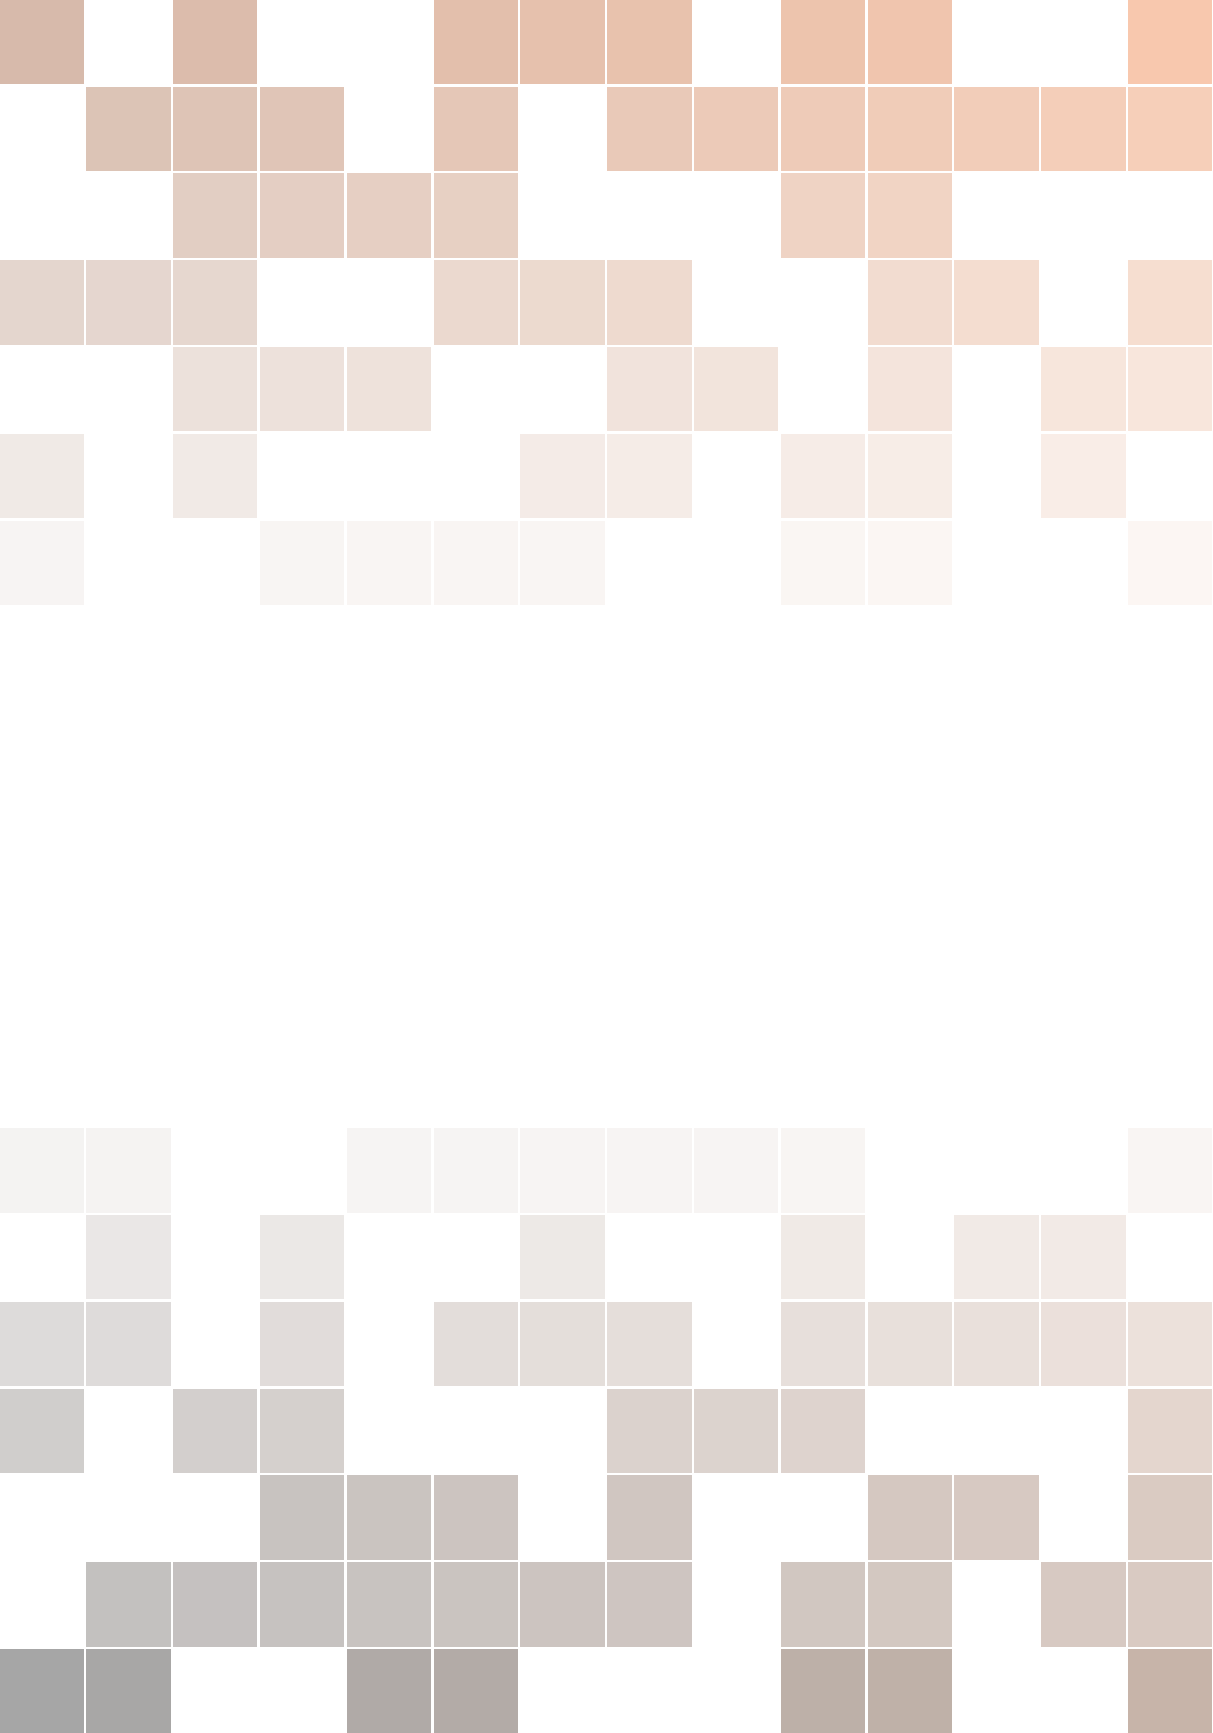
\includegraphics[width=\paperwidth]{background}}; % Background image
\draw[anchor=north] (midpoint) node [fill=ocre!30!white,fill opacity=0.6,text opacity=1,inner sep=1cm]{\Huge\centering\bfseries\sffamily\parbox[c][][t]{\paperwidth}{\centering STA247\\[15pt] % Book title
{\Large Probability with Computer Applications}\\[20pt] % Subtitle
{\huge Prof. K. H. Wong \\Sinan Li}}}; % Author name
\end{tikzpicture}};
\end{tikzpicture}
\vfill
\endgroup

%----------------------------------------------------------------------------------------
%	COPYRIGHT PAGE
%----------------------------------------------------------------------------------------

\newpage
~\vfill
\thispagestyle{empty}

\noindent Copyright \copyright\ 2013 John Smith\\ % Copyright notice

\noindent \textsc{Published by Publisher}\\ % Publisher

\noindent \textsc{book-website.com}\\ % URL

\noindent Licensed under the Creative Commons Attribution-NonCommercial 3.0 Unported License (the ``License''). You may not use this file except in compliance with the License. You may obtain a copy of the License at \url{http://creativecommons.org/licenses/by-nc/3.0}. Unless required by applicable law or agreed to in writing, software distributed under the License is distributed on an \textsc{``as is'' basis, without warranties or conditions of any kind}, either express or implied. See the License for the specific language governing permissions and limitations under the License.\\ % License information

\noindent \textit{First printing, March 2013} % Printing/edition date

%----------------------------------------------------------------------------------------
%	TABLE OF CONTENTS
%----------------------------------------------------------------------------------------

%\usechapterimagefalse % If you don't want to include a chapter image, use this to toggle images off - it can be enabled later with \usechapterimagetrue

\chapterimage{chapter_head_1.pdf} % Table of contents heading image

\pagestyle{empty} % No headers

\tableofcontents % Print the table of contents itself

\cleardoublepage % Forces the first chapter to start on an odd page so it's on the right

\pagestyle{fancy} % Print headers again

%----------------------------------------------------------------------------------------
%	PART 1
%----------------------------------------------------------------------------------------

\part{Contents}

\chapterimage{chapter_head_2.pdf} % Chapter heading image
\chapter*{Introduction} \addcontentsline{toc}{chapter}{Introduction}

This is an introductory course to probability, where our main focus will be developing an understanding of probability and the concept of probability distributions, both for discrete and continuous quantities. This includes developing the intuition for how probabilities `behave' and the situations in which it is valid to describe randomness using probability, as well as relying on simulations in R to help us visualize these properties.

By the end of the course, students should be able to...

\begin{itemize}
    \item Describe random quantities in various ways, such as by: their features, density functions, distribution functions, graphs
    \item Select an appropriate probability model based on their unique properties to quantify the randomness of random quantities
    \item Compute and interpret the various features of a random quantity: expected value, variance, standard deviation, correlation, covariance, event probabilities (either exactly, through approximations, or simulation)
    \item Select the most appropriate model to represent randomness and compute probabilities
    \item Use simulation in R for estimation purposes
    \item Explain the relationship of transforming a random variable and its effect on its distribution
    \item Use bivariate distributions to describe the association between two random quantities
\end{itemize}

\section*{Textbooks} \addcontentsline{toc}{section}{Textbooks}

We will be referencing these two textbooks regularly:

\begin{enumerate}
    \item \textit{Probability with Applications and R}, 2nd ed. by \textit{Wagaman and Dobrow} through the library \href{https://books-scholarsportal-info.myaccess.library.utoronto.ca/en/read?id=/ebooks/ebooks6/wiley6/2021-06-14/1/9781119692430#page=2}{here} and with student companion site \href{https://bcs.wiley.com/he-bcs/Books?action=index&itemId=1119692385&bcsId=12094}{here}.
    \item \textit{Modern Mathematical Statistics with Applications}, 3rd ed. by \textit{Devore and Berk} available through the library \href{https://login.library.utoronto.ca/index.php?url=https://link.springer.com/10.1007/978-3-030-55156-8}{here}.
\end{enumerate}

We will be using R throughout the course to help us understand probability distributions, and to simulate probabilities for quantities that are harder to compute by hand. R Markdown files will be provided for you with necessary starter code.  You'll also gain some experience with using \LaTeX to produce documents with well-presented math notation.

For new users to R, you may find chapters 3-7 from \href{https://r4ds.had.co.nz/}{R for Data Science} to be helpful as reference material in data visualization and data manipulation tools in R.

\section*{Course Information} \addcontentsline{toc}{section}{Course Information}

All course-related materials can be found on our Quercus page:

\begin{itemize}
    \item \textbf{Lectures} are held in MC 102 for both sections. We begin 10 minutes after the hour, and no recordings will be provided. 
    \item \textbf{Weekly materials} such as slides, suggested problems for practice, and reminders of upcoming due dates are posted each week's page on our course home page. 
    \item \textbf{Tutorial materials} will be distributed at the beginning of your tutorial. 
    \item \textbf{Announcements}: this is the primary channel to distribute important information to everyone! You're expected to check and read announcements regularly to ensure you don't miss any important communication! 
    \item \textbf{Assignments} and documents will be distributed and submitted through Crowdmark.
\end{itemize}

\section*{Discussion Board} \addcontentsline{toc}{section}{Discussion Board}

Throughout the term, beginning September 14, there will be pinned weekly discussions on our discussion board page. They will remain pinned from Wednesday 8 AM to the following Tuesday 8 PM.

\begin{itemize}
    \item \textbf{General Q\&A page}: general questions, clarifications, request for additional explanations, share your thoughts/understanding of topics 
    \item \textbf{Grouped practice problem discussions}: post your solutions, thoughts, approaches, questions here for that collection of textbook questions.
    \begin{itemize}
        \item Each discussion thread (i.e. reply to one original comment) is dedicated to ONE question, labeled in bold in the original comment
    \end{itemize}
\end{itemize}

You earn your discussion board credits by contributing at least five (5) times during this course to any of the discussions during the pinned period (Wednesday to Tuesday) in any of the following ways:

\begin{itemize}
    \item Posting a question to a problem you tried, with a clear explanation of your process, and if you got stuck: what you tried to do, and where you need help moving forward 
    \item Responding to a question with a thoughtful explanation to help your peer by sharing your own understanding of the problem 
    \item Posting to the general Q\&A page with your own question, about a course topic that is still unclear and being specific in describing what you do not understand (and perhaps what you did understand!) 
    \item Providing a detailed and clear response to a question in the general Q\&A page
\end{itemize}

To ensure boards are easy to reference, posting similar content is discouraged and these would be ineligible for earning credits.

\begin{itemize}
    \item Only contributions during the pinned period will be counted. The discussions will remain open the rest of term for students who come across new problems or would like to continue the discussions. 
    \item You are encouraged to keep the discussion going, but in terms of credit, it will be capped at 5 points. 
    \item While there is no weekly cap on points, the maximum points you can earn in the last two weeks is 2 points, with no more than 2 points per week (i.e. don't wait to the last minute to participate in the class discussion). 
    \item The discussion boards exist to facilitate peer-to-peer collaboration and learning, while also encouraging regular active engagement with course content. The course offers many opportunities that most students shouldn't find themselves unable to contribute in a unique way.
\end{itemize}

\subsection*{Why a Discussion Board?}

\begin{itemize}
    \item There are records and studies that have shown the process of explaining and teaching to others is an effective way to learn, consolidate, and retain what has been taught. See \href{https://digest.bps.org.uk/2018/05/04/learning-by-teaching-others-is-extremely-effective-a-new-study-tested-a-key-reason-why/}{here} and \href{https://scholar.princeton.edu/sites/default/files/cognition/files/impairment_effect.pdf}{here}.
    \item It's a space for students to come together to work collaboratively, receive and provide peer support. 
    \item It's also a space to get feedback and guidance from TAs and myself. 
    \item It's a good opportunity to self-assess (`how comfortable am I explaining this to another student?', `how often do I need to refer back to my notes to explain this concept clearly?') -- an important component of good study skills! 
    \item It's valuable information to us! Common questions/misunderstandings that pop up in the weekly discussions can be addressed during our weekly lecture meetings.
\end{itemize}

\subsection*{Discussion Board Rubric}

\begin{center}
    \begin{tabular}{ | p{0.1\linewidth} | p{0.25\linewidth} | p{0.25\linewidth} | p{0.25\linewidth} | }
        \hline
        Points & 1 point & 0.5 points & 0 points \\
        \hline
        Quality of contribution & Student has made a substantial and unique contribution with detailed explanations and/or clearly outlined process of the approach to a problem. & Student has made a contribution to the discussion that is dismissive, lacking in detail, or not completely unique. Unable to further the discussion in a way that fosters a collaborative learning environment. & Student has not contributed to the weekly discussion topic thread, or whose posts are off-topic/irrelevant/do not contribute to the thread or is not unique to what has already been discussed in the thread. \\ & & & \\
        & Student was involved in follow-up discussions and worked collaboratively with their peers to develop a better understanding of the concepts involved. & e.g. responses such as `you just need to integrate this and solve for it' or `I got the same answer doing... (reiterates OPs process)' & e.g. `I got the same answer', `How did you get that number?' \\
        \hline
    \end{tabular}
\end{center}

\subsection*{Tutorial}

\begin{itemize}
    \item A mix of R labs and collaborative pair work 
    \item R labs: These labs have guided exercises to practice the R tools covered in class or learn new R skills. Labs will be TA-guided. 
    \item R labs require individual .rmd and knitted document submissions at the end of tutorial (Note that the labs are guided and meant to be completed within the tutorial time) 
    \item Pair work: In your tutorial section, you will with a partner of your choice work on more challenging but guided problems together. Discussion and sharing your ideas is a great way to learn from one another, and consider different approaches to problem solving! TAs will be there to support and help answer clarification questions.
\end{itemize}

\subsection*{Habits for Success}

\begin{itemize}
    \item Attend and participate in lecture. Try to work along with the problems presented. Ask questions and interact with your peers during the open work periods! 
    \item Make sure you focus on \textit{understanding} the concepts and how they relate and build upon each other. This one is hard! 
    \item Regularly attempt as many of the suggested problems as you can and work towards being able to work on the problems closed book. Use this to gauge your familiarity with the material -- if it takes you an hour to work through two problems, then it's a good indication to seek out advice and support from the teaching team. The earlier, the better! 
    \item Drop by during the office hours or post on discussion board if you get stuck. Work through practice problems with classmates. Take turns \textit{explaining} your thinking and problem solving process. 
    \item \textbf{Create a schedule and stick with it}. This course covers many topics to ensure you have a good foundation for latter courses. Many topics build on top of each other so falling behind can quickly snowball and make it difficult to catch up.
\end{itemize}

\textbf{Some Suggestions from Previous Students}

\begin{enumerate}
    \item Will the final be cumulative?

    Yes. 
    
    \item I find that I \textit{really} struggle with keeping my mind focused on the question I'm presenting working on, and not think about how a similar question was solved previously. I thought I was making some progress, but then I realized this wasn't the case at all after today when I spent 30 minutes trying to recall the solution I wrote for A2 (I don't remember even reading the test question..I just caught a few phrases and began regurgitating my assignment solution incorrectly).

    I realize the most helpful thing I can do for myself now is to practice regularly, but I can't say I've been doing that well. For the last week, I've been attempting the textbook questions (open book )in preparation for the test. For the final, I plan to solve questions independently, which was something I didn't do until last minute. What else can I do to improve my problem-solving/critical thinking skills?

    Definitely do textbook / slide questions closed book. The only thing you should be looking at is the sample aid sheet. Otherwise you will never know if you actually understand the material.

    \item You need to know when you don't know something. Meaning that when you see a question, you need to recognize if you actually know how to solve it or not. And if you don't know how to solve it you need to skip it and go to the next question. I'm sure you know that spending 30 min on any question is not an efficient use of the time.  
    
    \item Go to office hours. There is only like 2 other people that I've ever seen at office hours.
    
    \item What does data have to look like for an exponential distribution to describe it?

    Why do we use different distributions? What's the importance of justifying a decision to use one distribution over another? (the textbook often tells you the distribution so image all of the questions posed to you without that information. Would you still be confident?) Answering these questions thoroughly will make you a lot better at figuring out how to approach a question when you see it.

    Understanding the conceptual side in depth is the most important part of studying I would think. Computational skills come with practice, eventually you get it. But usually the problem with stats or courses like this is interpreting the question - is figuring out how to even approach the question in the first place. Knowing how to solve all of the normal distribution questions that confront you is great, but that won't help you if you can't even recognize when and when not to use it.
\end{enumerate}

\chapterimage{chapter_head_2.pdf}
\chapter{Introduction to Probability}

\section{Useful Terminology}

\begin{definition}[Random Experiment]\index{Random Experiment}
    A process that allows us to gather data or observations. Experiment can be repeated multiple times under the same conditions. The set of possible outcomes of the experiment are known, but the outcome of a specific experiment is not known.
\end{definition}

\begin{example}
    Below are some examples of random experiments. 

    \begin{itemize}
        \item Rolling a die and observing the top-facing number 
        \item Rolling a pair of dice and observing the sum of top-facing numbers 
        \item A patient being administered a painkiller and observing the amount of time in minutes before relief is felt
    \end{itemize}
\end{example}

\begin{definition}[Sample Space]\index{Sample Space}
    
\end{definition}

\chapterimage{chapter_head_2.pdf}
\chapter{Counting}

\section{Counting and Probability}

\begin{proposition}[Probability as Relative Frequency]
    The long-run relative frequency of an event $A$ will approach the probability of event $A$. In cases where the sample space consists of \bred{equally likely} elements, we can find this probability by calculating the relative frequency of $A$ in $\Omega$ by $$P(A) = \frac{\text{Number of outcomes in } A}{\text{Total number of possible outcomes in the random experiment}} = \frac{n(A)}{n(\Omega)}$$
    This is valid \bred{only if} each element in $\Omega$ is \bred{equally likely}. 
\end{proposition}

\section{Fundamental Principle of Counting}

Experiments that involve equally likely discrete outcomes make calculating probabilities much easier when we have methods to count outcomes.

\begin{itemize}
    \item For an experiment with two events of interest, $A$ and $B$, you can use the Inclusion-Exclusion Principle to count the number of outcomes in event $A \cup B$: $n(A \cup B) = n(A) + n(B) - n(A \cap B)$, where $n(X)$ denotes the number of elements in event $X$. 

    \item For experiments that involve \itblue{multiple \bred{ordered}} stages, we can use the \bred{Fundamental Principle of Counting} (FPC) to count the number of unique outcomes from this multi-stage experiment. 
\end{itemize}

\begin{example}[Toy Example]
    A new sandwich shop seems to only have limited customization options. They offer three types of greens (lettuce, spinach, mixed greens), five types of deli meat, and four types of cheese. Sandwiches are built by layering with greens, followed by deli meat, and topping it off with cheese. How many unique sandwiches can be created if a customer randomly chooses one of each item to include in their sandwich?

    This experiment involves $3$ ordered stages:
    \begin{itemize}
        \item Stage 1: Pick a green - $3$ choices
        \item Stage 2: Pick a deli meat - $5$ choices
        \item Stage 3: Pick a cheese - $4$ choices
    \end{itemize}

    Each option is equally likely to be chosen since we're considering all possible combinations

    There are in total $3 \times 5 \times 4 = 60$ unique combinations. 
\end{example}

When counting the number of (ordered) outcomes from a multistage experiment, we can use the Fundamental Principle of Counting.

\begin{theorem}
    If an experiment consists of $m$ (\bred{ordered}) stages with $n_1$ possible outcomes in stage 1, $n_2$ possible outcomes in stage 2, $\dots$, $n_m$ possible outcomes in stage $m$, then the total number of possible outcomes is $$\prod_{i=1}^m n_i$$
\end{theorem}

\section{Permutation}

\begin{example}
    FPC counts specifically \bred{ordered stages}. In the toy example, the number of sandwiches only include those that are layered in a specific order: with greens on the bottom, then deli meat, then cheese on top. However, customers might have a preference for how the ingredients are layered. 

    \begin{enumerate}[label=\alph*)]
        \item How many different ways can the ingredients (greens, deli meat, cheese) be layered/permuted?

        \begin{itemize}
            \item Stage 1: 3 choices
            \item Stage 2: 2 choices
            \item Stage 3: 1 choice
        \end{itemize}

        There are in total $3 \times 2 \times 1 = 6$ ways. 

        \item If the choice and order of ingredients each result in a `different' sandwich, how many sandwich choices are there?
        
        $6$ choices to order ingredients $\times 60$ ingredient combinations $= 360$ `different' sandwiches. 
    \end{enumerate}
\end{example}

\begin{definition}[Permutation - $_nP_n$]
    The number of ways to order $n$ \bred{distinct} item is $$n! = n \times (n - 1) \times \cdots \times 2 \times 1$$
\end{definition}

\begin{definition}[Permutation - $_nP_k$]\index{Permutation}
    The number of ways to select \itblue{ordered subset} of $k$ elements from a group of $n$ \bred{distinct} items is $$_nP_k = \frac{n!}{(n-k)!}$$
\end{definition}

The intuition behind this formula is to count all possible arrangements ($n!$) and group together all arrangements that have the same objects in the first $k$ stages. The resulting number of `groups' is the number of unique ordered subset. The number of elements in each group is equivalent to the number of ways to arrange the remaining $(n - k)$ objects. 

\chapterimage{chapter_head_2.pdf}
\chapter{Conditional Probability}

\section{Conditional Probability}

\begin{example}[Thought Exercise]
    For the following, assume that the probability of having a child of either sex (male or female) is $50\%$.

    \begin{enumerate}[label=\alph*)]
        \item A family has two children. What are the chances this family has two boys? 

        $\Omega = \{ BB, BG, GB, GG \}$

        $P(BB) = \frac{1}{4}$

        \item A family has two children, and you know that one of the children is a boy. What are the chances this family has two boys?
        
        $\Omega = \{ BB, BG, GB \}$

        $P(\text{2 boys if one boy}) = \frac{1}{3}$
    \end{enumerate}
\end{example}

\begin{example}
    Below is a contingency table of counts in a fictional study of colourblindness among the two sexes. $C$ denotes the event that a surveyed individual is colourblind, and $M$ denotes the event that a surveyed individual is male.

    \begin{center}
        \begin{tabular}{c | c c | c}
                          & $C$   & $C^c$  & Row Totals \\
            \hline
            $M$           & $106$ & $1175$ & $1281$     \\
            $M^c$         & $7$   & $1212$ & $1219$     \\
            \hline
            Column Totals & $113$ & $2397$ & $2500$
        \end{tabular}
    \end{center}

    \begin{enumerate}[label=\alph*)]
        \item What is the estimated probability that an individual is male and colourblind?

        $\begin{aligned}[t]
            P(M \cap C) & = \frac{n(M \cap C)}{n(\Omega)} \\
                        & = \frac{106}{2500}              \\
                        & \approx 4.52 \%
        \end{aligned}$

        \item What is the estimated probability that a male individual is colourblind? That a female individual is colourblind?

        \begin{minipage}[t]{0.45\linewidth}
            $\begin{aligned}[t]
                P(C \text{ if } M) & = \frac{n(C \cap M)}{n(M)} \\
                                   & = \frac{106}{1281}         \\
                                   & \approx 8.27 \%
            \end{aligned}$

            $\therefore 8.27\%$ of males surveyed reported to be colourblind. 
        \end{minipage}
        \hspace{0.025\linewidth}
        \begin{minipage}[t]{0.45\linewidth}
            $\begin{aligned}[t]
                P(C \text{ if } M^c) & = \frac{n(C \cap M^c)}{n(M^c)} \\
                                     & = \frac{7}{1219}               \\
                                     & \approx 0.57 \%
            \end{aligned}$

            $\therefore 0.57\%$ of females surveyed reported to be colourblind. 
        \end{minipage}
    \end{enumerate}
\end{example}

\begin{definition}[Conditional Probability]\index{Conditional Probability}
    The notation $P(A | B)$ denotes the probability that of event $A$ under the condition that event $B$ is known to have occurred. $$P(A | B) = \frac{P(A \cap B)}{P(B)} \quad \text{provided that } \color{red} P(B) > 0$$
\end{definition}

Rearranging the above, we have the following relations we can use depending on available information $$P(A \cup B) = P(A | B) \cdot P(B) \qquad \text{ or } \qquad P(A \cup B) = P(B | A) \cdot P(A)$$

Conditional probabilities provide additional information when we know partially the outcome of a random experiment. Conditional probabilities are probability distributions on a \bred{restricted sample space}, and follow the same probability
axioms.

\begin{axiom}
    Consider a random experiment with sample space $\Omega$. Let $B$ be an event ($B \subseteq \Omega$) with $P(B) > 0$. Let $b$ denote the elements of event $B$. Than, 

    \vspace{0.5em}
    \begin{enumerate}
        \item $P(b | B) \ge 0$ for all $b \in B$. 
        \vspace{0.5em}
        \item $\sum_{b \in B} P(b | B) = 1$
        \item For $A \subseteq B$, $P(A | B) = \sum_{b \in A} P(b | B)$
    \end{enumerate}
\end{axiom}

Some examples include 
\begin{itemize}
    \item determining the probability distribution of disease status when someone tests negative for a disease 
    \item applications in Bayesian statistics, Bayes classification, etc.
\end{itemize}

\begin{example}
    You pick a card at random from a standard deck of cards. Define events Q where a queen of hearts is drawn and R where a red card is drawn. Describe the events below and find their probabilities.

    \begin{enumerate}[label=\alph*)]
        \item $Q | R$
        
        $\begin{aligned}[t]
            P(Q | R) & = \frac{P(Q \cap R)}{P(R)}             \\
                     & = \frac{\sfrac{1}{52}}{\sfrac{26}{52}} \\
                     & = \frac{1}{26}
        \end{aligned}$

        \item $R | Q$

        $\begin{aligned}[t]
            P(R | Q) & = \frac{P(R \cap Q)}{P(R)}            \\
                     & = \frac{\sfrac{1}{52}}{\sfrac{1}{52}} \\
                     & = 1
        \end{aligned}$

        \item $Q^c | R$ 
        
        $\begin{aligned}[t]
            P(Q^c | R) & = 1 - P(Q | R)     \\
                       & = 1 - \frac{1}{26} \\ 
                       & = \frac{25}{26}
        \end{aligned}$
    \end{enumerate}
\end{example}

\section{Independence}

Recall that two events are independent if the occurrence of one (A) does not alter the chances of the other event (B). Formally, we have the following.

\begin{definition}[Independent Events]\index{Independent Events}
    Two events $A$ and $B$ are \term{independent} if 
    $$P(A | B) = P(A) \qquad \text{provided that } P(B) > 0$$
    $$P(B | A) = P(B) \qquad \text{provided that } P(A) > 0$$

    Using this, we can show that event $A$ is independent of event $B$, then $P(A \cap B) = P(A) \cdot P(B)$. Otherwise, the two events are dependent. 
\end{definition}

\begin{definition}[Mutually Exclusive]\index{Mutually Exclusive}
    Two events are \term{mutually exclusive} if the occurrence of one ($A$) excludes the occurrence of the other ($B$). Event-wise, the two sets are disjoint ($A \cap B = \emptyset$) and $P(A \cap B) = 0$. This implies that the events are dependent.
\end{definition}

For example, given $P(A) > 0$ and $P(B) > 0$, $A$ and $B$ are mutually exclusive when $P(A | B) = P(B | A) = 0$.

{~~~}

If events $A$ and $B$ are independent, then so are their complements $A^c$ and $B^c$. 

{~~~}

For a collection of $n$ events, $A_1$, $A_2$, $\dots$, $A_n$, 

\begin{itemize}
    \item If all $n$ events are independent, then $$P(A_1 \cap A_2\ cap \cdots \cap A_n) = P(A_1) \times P(A_2) \times \cdots \times P(A_n)$$
    \item $A_1, \dots, A_n$ are \bred{mutually independent} if for any subset of $k$ events, $k = 2, 3, \dots, n$< $$P(A_{i_1} \cap A_{i_2} \cap \cdots \cap A_{i_k}) = P(A_{i_1}) \times P(A_{i_2}) \times \cdot \times P(A_{i_k})$$
\end{itemize}

\begin{example}
    Two events $E$ and $F$ have the properties $P(E) = 0.44$, $P(F) = 0.6$, and $P(E \cap F) = 0.35$. Use the information to determine whether events $E$ and $F$ are independent. 

    \begin{minipage}[t]{0.45\linewidth}
        $\begin{aligned}[t]
            P(E | F) & = \frac{P(E \cap F)}{P(F)} \\
                     & = \frac{0.35}{0.6}         \\
                     & \approx 0.5933
        \end{aligned}$
    \end{minipage}
    \begin{minipage}[t]{0.45\linewidth}
        $\begin{aligned}[t]
            P(E) \times P(F) & = 0.44 \times 0.06 \\
                             & = 0.264
        \end{aligned}$
    \end{minipage}

    Clearly, $P(E | F) \neq P(E) \times P(F)$. $E$ and $F$ are NOT independent. 
\end{example}

\begin{example}
    A system below is made of independent components. The probability that the first component works is $0.9$, $0.95$ for the second component, and $0.99$ for the third component. The signal can travel from left to right if there is a circuit made of working components. Find the probability that the signal is blocked.

    \begin{center} 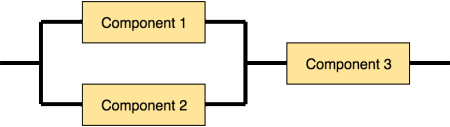
\includegraphics[width=0.5\linewidth]{IndependentEventsExample2.png} \end{center}

    Let $B$ be the event that the signal is blocked. Let $C_1$, $C_2$ and $C_3$ be the events that components $1$, $2$, and $3$ are working. 

    $\begin{aligned}[t]
        P(B) & = P({C_3}^c \cup ({C_1}^c \cap {C_2}^c))                                                     \\
             & = P({C^3}^c) + P({C_1}^c \cap {C_2}^c) - P({C_1}^c \cap {C_2}^c \cap {C_3}^c)                \\
             & = P({C^3}^c) + P({C_1}^c) \times P({C_2}^c) - P({C_1}^c) \times P({C_2}^c) \times P({C_3}^c) \\
             & = 0.01 + 0.1 \times 0.05 - 0.1 \times 0.05 \times 0.01                                       \\
             & = 1.495 \%
    \end{aligned}$
    
    {~~~}

    Alternatively, we can the the indirect method. 

    $\begin{aligned}[t]
        P(B) & = 1 - P(B^c)                                                                                                                    \\
             & = 1 - P(C_3 \cap (C_1 \cup C_2))                                                                                                \\
             & = 1 - P((C_3 \cap C_1) \cup (C_3 \cap C_2))                                                           & \text{distribution law} \\
             & = 1 - \left( P(C_1 \cap C_3) + P(C_2 \cap C_3) - P(C_1 \cap C_2 \cap C_3) \right)                                               \\
             & = 1 - \left( P(C_1) \times P(C_3) + P(C_2) \times P(C_3) - P(C_1) \times P(C_2) \times P(C_3) \right)                           \\
             & = 1 - (0.9 \times 0.99 + 0.95 \times 0.99 - 0.9 \times 0.95 \times 0.99)                                                        \\
             & = 1 - 0.98505                                                                                                                   \\
             & = 1.495 \%
    \end{aligned}$
\end{example}

\section{Bayes' Rule}

Given two events, we know that their conditional probability is defined as $$P(A | B) = \frac{P(A \cap B)}{P(B)} \qquad \text{provided that } P(B) > 0$$ which can be rearranged to $$P(A \cap B) = P(A | B) \cdot P(B)$$

Suppose now we have a sample space consisting \bred{only} of events $A, B_1, B_2, \dots, B_k$ where the $B_i$'s \bred{partitions the sample space}. That is, the $B_i$'s are disjoint and $\bigcup_{i=1}^k B_i = \Omega$. From Axiom 3, we can show that $$P(A) = P(A \cap B_1) + P(A \cap B_2) + \cdots + P(A \cap B_k)$$ Combining this with our knowledge of conditional probability, we get the \bred{Law of Total Probability}.

\begin{theorem}[Law of Total Probability]\index{Law of Total Probability}
    If $B_1, B_2, \dots, B_k$ is a collection of mutually exclusive (disjoint) and exhaustive events that partition the sample space, then for any event $A$, $$P(A) = \sum_{i=1}^n P(A | B_i) \cdot P(B_i)$$
\end{theorem}

Putting together the Law of Total Probability and definition of conditional probability, we get \bred{Bayes' Rule}. 

\begin{theorem}[Bayes' Rule]\index{Bayes' Rule}
    Let $B_1, B_2, \dots, B_k$ form a partition of the sample space and let $A$ be an event in $\Omega$. Than $$\begin{aligned}[t]
        P(B_i | A) & = \frac{P(A \cap B_i)}{P(A)}                                           \\
                   & = \frac{P(A | B_i) \cdot P(B_i)}{\displaystyle \sum_{i=1}^k P(A | B_i) \cdot P(B_i)}
    \end{aligned}$$
\end{theorem}

\begin{example}
    A ball is drawn at random from an urn containing one red and one white ball. If the white ball is drawn, it is put back into the urn. If the red ball is drawn, it is returned to the urn together with two more red balls. Then a second draw is made.

    \begin{enumerate}[label=\alph*)]
        \item What is the probability a red ball was drawn on both the first and the second draws?

        Let $W_i$ be the event where a white ball is drawn on the $i$\textsuperscript{th} draw. 

        Let $R_i$ be the event where a red ball is drawn on the $i$\textsuperscript{th} draw. 

        $\begin{aligned}[t]
            P(R_1 \cap R_2) & = P(R_1) \times P(R_1 | R_1)     \\
                            & = \frac{1}{2} \times \frac{3}{4} \\
                            & = \frac{3}{8}
        \end{aligned}$

        \item What is the probability that a red ball was drawn first if the second ball drawn was red?

        \begin{minipage}[t]{0.35\linewidth}
            \begin{center}
                \tikzsetnextfilename{c03s03-01}
                \begin{tikzpicture}[baseline=(current bounding box.north)]
                    \draw (-1,-1) node {$W_1$};
                    \draw (1,-1) node {$R_1$};
                    %
                    \draw (-1.5,-2) node {$W_2$};
                    \draw (-0.5,-2) node {$R_2$};
                    \draw (0.5,-2) node {$W_2$};
                    \draw (1.5,-2) node {$R_2$};
                    %
                    \draw (0,0) -- (-0.7,-0.7) node[above] {$\sfrac{1}{2}$};
                    \draw (0,0) -- (0.7,-0.7) node[above] {$\sfrac{1}{2}$};
                    %
                    \draw (-1,-1.3) -- (-1.5,-1.7) node[above] {$\sfrac{1}{2}$};
                    \draw (-1,-1.3) -- (-0.5,-1.7) node[above] {$\sfrac{1}{2}$};
                    \draw (1,-1.3) -- (0.5,-1.7) node[above] {$\color{red} \sfrac{1}{4}$};
                    \draw (1,-1.3) -- (1.5,-1.7) node[above] {$\color{red} \sfrac{3}{4}$};
                \end{tikzpicture}
            \end{center}
        \end{minipage}
        \begin{minipage}[t]{0.6\linewidth}
        $\begin{aligned}[t]
            P(R_1 | R_2) & = \frac{P(R_1 \cap R_2)}{P(R_2)}                                                           \\
                         & = \frac{\sfrac{3}{8}}{P(R_1 \cap W_1) + P(R_2 \cap R_1)}                                   \\
                         & = \frac{\sfrac{3}{8}}{P(R_2 | W_1) \times P(W_1) + P(R_2 | R_1) \times P(R_1)}             \\
                         & = \frac{\sfrac{3}{8}}{\sfrac{1}{2} \times \sfrac{1}{2} + \sfrac{3}{4} \times \sfrac{1}{2}} \\
                         & = \frac{3}{5}                                                                              \\
                         & = 60\%
        \end{aligned}$
        \end{minipage}
        
    \end{enumerate}
\end{example}

\begin{example}
    Consider HIV testing. An HIV test will correctly test positive $95\%$ of the time (sensitivity), and incorrectly test positive $1\%$ (false positive rate) of the time. Suppose we know that $99.99\%$ of the population is HIV-free. Under these conditions, what is the probability that a patient who tested positive is actually HIV positive?

    \begin{minipage}[t]{0.4\linewidth}
        \begin{center} 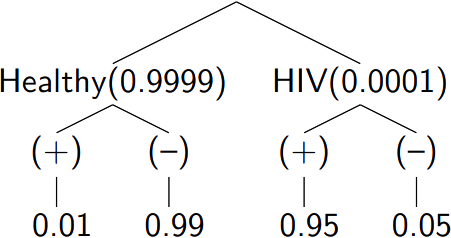
\includegraphics[width=0.75\linewidth,valign=t]{BayesRuleExampleHivTesting.png} \end{center}
    \end{minipage}
    \begin{minipage}[t]{0.55\linewidth}
        $\begin{aligned}[t]
            P(\text{HIV} | +) & = \frac{P(\text{HIV} \cap +)}{P(+)} \\
            & = \frac{P(\text{HIV} \cap +)}{P(+ \cap \text{Healthy}) + P(+ \cap \text{HIV})} \\
            & = \frac{0.95 \times 0.0001}{0.01 \times 0.9999 + 0.95 \times 0.0001} \\
            & = 0.94\%
        \end{aligned}$
    \end{minipage}

    $\therefore$ If we were randomly pick a person and test them for HIV, there chance of them having HIV with a positive test is $0.94\%$. 
\end{example}

\chapterimage{chapter_head_2.pdf}
\chapter{Discrete Distributions}

\section{Random Variables}

\subsection{Introduction to Random Variables}

\begin{definition}[Random Variable]\index{Random Variable}
    A \term{random variable} is a real-valued function that assigns a numerical value to each event in the sample space $\Omega$ arising from a random experiment. A random variable $X$ is a \bred{real-valued function} $X : \Omega \to \mathbb{R}$ such that for every $\omega \in \Omega$, $X(\omega) = x \in \mathbb{R}$. It is a mapping from the sample space to the real numbers.
\end{definition}

\begin{example}
    Consider the random experiment of tossing a coin. 

    \begin{itemize}
        \item $\Omega = \{ H, T \}$
        \item Let $X$ be the RV denoting the outcome of a toss. We ca define $X$ such that $X(H) = 1$, $X(T) = 0$ essentially converting each outcome into a number. 
        \item By convention, we will denote random variables with capital letters, and a particular (unknown value) of a random variable with its lower case equivalent. i.e. for a random variable $X$, a particular value of this RV would be denoted by $x$.
    \end{itemize}
\end{example}

\begin{definition}[Discrete Random Variable]\index{Discrete Random Variable}\index{Continuous Random Variable}
    A \term{discrete} of a random variable $X$ is one tha can take on only a finite number of a countably infinite number of possible values $x$. A random variable $X$ is \term{continuous} if its domain is an interval of real numbers. 
\end{definition}

\begin{definition}[Probability Mass Function]\index{Probability Mass Function}
    A \term{probability mass function} (PMF) of a discrete random variable is one that assigns a probability to each value $x \in C$ such that 
    \begin{itemize}
        \item $0 \le P(X = x) \le 1$
        \item $\sum_{x \in X} P(X = x) = 1$
    \end{itemize}
\end{definition}

\begin{example} 
    Below are some examples of random variables. 

    \textbf{Discrete RV Examples}
    
    \begin{itemize}
        \item The number of defects in a day's production of car parts 
        \item The number of new arrivals in a queue 
        \item The status of your internet service: online or offline 
        \item The number of students online at a particular time
    \end{itemize}

    \textbf{Continuous RV Examples}

    \begin{itemize}
        \item The weight of a randomly selected individual 
        \item The time it takes to load a video 
        \item The temperature in the morning of a random day
    \end{itemize}
\end{example}

\begin{example}
    Determine the value of $k$ such that $f(x) = \frac{kx^2 - x + 2}{4}$ will be a valid probability mass function for $X = \{ 0, 1, 2, 3, 4 \}$.

    \begin{center}
        \begin{tabular}{c | c c c c c}
            $X$        & 0             & 1               & 2              & 3                & 4                 \\
            \hline
            $P(X = x)$ & $\frac{2}{4}$ & $\frac{k+1}{4}$ & $\frac{4k}{4}$ & $\frac{9k-1}{4}$ & $\frac{16k-2}{4}$
        \end{tabular}
    \end{center}

    We need $\sum_{x=0}^4 P(X = x) = 1$. That is, 
    $\begin{aligned}[t]
        \frac{2 + (k+1) + (4k) + (9k-1) + (16k-2)}{4} & = 1            \\
        30k                                           & = 4            \\
        k                                             & = \frac{2}{15}
    \end{aligned}$

    Thus, $k$ must be $\frac{2}{15}$ for $\sum_{x \in X} P(X = x) = 1$. 

    \begin{center}
        \begin{tabular}{c | c c c c c}
            $X$        & 0             & 1               & 2              & 3              & 4              \\
            \hline
            $P(X = x)$ & $\frac{1}{2}$ & $\frac{17}{60}$ & $\frac{2}{15}$ & $\frac{1}{20}$ & $\frac{1}{30}$
        \end{tabular}
    \end{center}
\end{example}

\begin{example}
    A factory producing computer parts sends out a shipment of $10$ parts of which $3$ are defective. Find the probability mass function for the number of defectives a customer will get if the first customer randomly purchases $4$ computer parts.

    Let $D$ be the number of defectives purchased. 

    $D = \{ 0, 1, 2, 3 \}$. 

    \begin{itemize}
        \item $P(D = 0) = \frac{_7C_4}{_{10}C_4}$
        \item $P(D = 1) = \frac{_3C_1 \times _7C_3}{_{10}C_4}$
        \item $P(D = 1) = \frac{_3C_2 \times _7C_2}{_{10}C_4}$
        \item $P(D = 1) = \frac{_3C_3 \times _7C_1}{_{10}C_4}$
    \end{itemize}

    We may conclude that $P(D = d) = \frac{_3C_d \times _7C_{4-d}}{_{10}C_4}$. 
\end{example}

\begin{example}
    A quiz consists of $10$ true/false problems. A student takes the quiz by randomly selecting the answers. Examine the graph of the probability mass function and describe the behaviour of the random number of correct answers X.

    For discrete distribution, we use bar charts. The bins are $0, 1, 2, 3, \dots, 10$, which are discrete. Histograms, on the other hand, has bins that span a continuous interval, for example, $[0, 1), [1, 2), [2, 3), \dots$. 

    \begin{itemize}
        \item $4, 5, 6$ have the highest probability mass, meaning they are the most \itblue{likely}; 
        \item $0, 1, 2, 8, 9, 10$ have the lowest probability mass, meaning that they are the most \itblue{unlikely};
        \item $3$ and $7$ lie between \itblue{likely} and \itblue{unlikely}.
    \end{itemize}

    \begin{center} 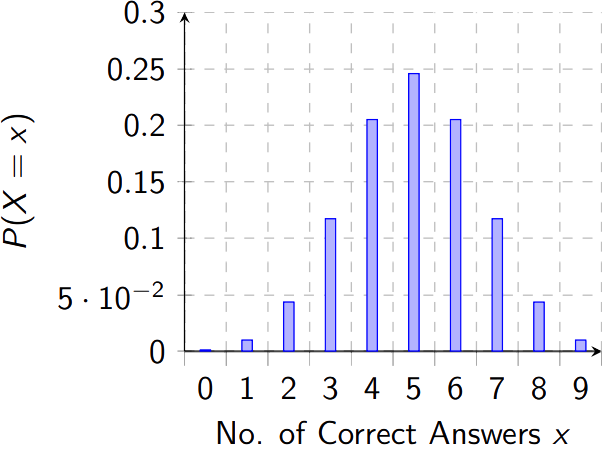
\includegraphics[width=0.5\linewidth]{PmfExamplesTFQuiz.png} \end{center}
\end{example}

\subsection{Characteristics of Random Variables}

Both the PMF and CDF describe the exact distribution of a random quantity. Distributions have two useful characteristics that are often used in statistics:

\begin{itemize}
    \item \term{Expected Value}: The long run/theoretical average. If a random experiment were to be conducted $n$ times, then as $n \to \infty$ then the average of outcomes converges to the expected value. This is often denoted as $\mu$.
    \item \term{Variance} or \term{Standard Deviation}: Are measures of the spread and variability of a random variable. Standard deviation is the square root of variance. Variance is often denoted as $\sigma^2$ and SD as $\sigma$.
\end{itemize}

\begin{definition}[Expected Value]\index{Expected Value}
    The \term{expected value} of a discrete random quantity $X$ is defined to be $$\mu = E(X) = \sum_{x \in X} x \cdot P(X = x)$$

    For a given transformation of $X$, $g(X)$, $E(g(x))$ can be found by $$E(g(x)) = \sum_{x \in X} g(x) \cdot P(X = x)$$

    Note that $E(g(x)) \neq g(E(X))$ except when $g(X)$ is a linear transformation. 
\end{definition}

\textbf{Review of Summation Rules}

\begin{itemize}
    \item $\sum_{i=1}^n c = n \cdot c$ for a constant $c$
    \item $\sum_{i=1}^n c \cdot x_i = c \cdot \left( \sum_{i=1}^n x_i \right)$
    \item $\sum_{i=1}^n i = \frac{n \cdot (n+1)}{2}$
\end{itemize}

\begin{example}
    A mining company needs a type of drill bit for a project. It is known through historical data that these drill bits for similar projects will last $2$, $4$, or $7$ hours with probabilities $0.1$, $0.7$, and $0.2$. How long do they expect each drill bit to last, on average?

    Let $L$ be the longevity of a random drill bit.

    \begin{center}
        \begin{tabular}{c | c c c}
            $l$        & 2     & 4     & 7     \\
            \hline
            $P(L = l)$ & $0.1$ & $0.7$ & $0.2$
        \end{tabular}
    \end{center}

    $\begin{aligned}[t]
        E(L) & = \sum_{l \in L} l \cdot P(L = l)         \\
             & = 2 \cdot 0.1 + 4 \cdot 0.7 + 7 \cdot 0.2 \\
             & = 4.4 \text{ hours}
    \end{aligned}$

    $\therefore$ on average, the drill bits will last $4.4$ hours.
\end{example}

\textbf{Properties of Expectation}

For any constants $a$, $b$, and discrete variables $X$, the following are true.

\begin{itemize}
    \item $E(a) = 0$

    \item $E(X + a) = E(X) + a = \mu + a$. 

    Increase in $x \in X$ will shift the centre / average by the same amount. 

    \item $E(aX) = a \cdot E(X) = a \cdot \mu$
    
    \begin{proof}
        Take $g(X) = aX$. Then, $\begin{aligned}[t]
            E(g(x)) & = \sum_{x \in X} g(x) \cdot P(X = x) \\
                    & = \sum_{x \in X} ax \cdot P(X \in x) \\
                    & = a \sum_{x \in X} x \cdot P(X = x)  \\
                    & = a \cdot \color{red} E(x)           \\
                    & = a \cdot \mu
        \end{aligned}$
        
        That is, $E(aX) = a \cdot E(X) = a \cdot \mu$. 
    \end{proof}

    \item $E(aX + b) = a \cdot E(X) + b = a \cdot \mu + b$

    \begin{proof}
        Take $g(X) = aX + b$. $g(x)$ is a linear transformation of $X$. 

        $E(g(x)) = g(E(x))$ if $g(X)$ is a linear transformation of $X$. 
        
        Thus, $E(aX + b) = a \cdot E(X) + b = a \cdot \mu + b$. 
    \end{proof}

    \item $E(X + Y) = E(X) + E(Y)$. 

    \item $E(XY) \neq E(x) \cdot E(Y)$ \bred{unless} $X$ and $Y$ are \itblue{independent}. 
\end{itemize}

\begin{definition}[Variance]\index{Variance}\index{Standard Deriviation}
    For a discrete variable $X$, the \term{variance} of $X$ is defined to be $$\sigma^2 = V(X) = E((X - \mu)^2) = \sum_{x \in X} (x - \mu)^2 \cdot P(X = x)$$ 
    Variance captures the spread in $units^2$. The standard deviation, $\sigma = \sqrt{\text{variance}}$ is a measure of spread in the same units as the random variable $X$. 
\end{definition}

\begin{example}
    A mining company needs a type of drill bit for a project. It is known through historical data that these drill bits for similar projects will last $2$, $4$, or $7$ hours with probabilities $0.1$, $0.7$, and $0.2$. Find the variance and standard deviation in the longevity of this type of drill bit. Interpret the values

    Let $L$ be the longevity of a random drill bit.

    We also found $\mu = 4.4$

    \begin{center}
        \begin{tabular}{c | c c c}
            $l$           & 2                & 4                & 7                \\
            \hline
            $P(L = l)$    & $0.1$            & $0.7$            & $0.2$            \\
            $(l - \mu)^2$ & $(2-4.4)^2=5.76$ & $(4-4.4)^2=0.16$ & $(7-4.4)^2=6.76$
        \end{tabular}
    \end{center}

    $\begin{aligned}[t]
        V(L) & = {\sigma_L}^2                                         \\
             & = \sum_{l \in L} (l - \mu)^2 \cdot P(L = l)        \\
             & = 5.76 \cdot 0.1 + 0.16 \cdot 0.7 + 6.76 \cdot 0.2 \\
             & = 2.04 \text{ hours}^2
    \end{aligned}$

    Then, $\begin{aligned}[t]
        SD(L) = \sqrt{V(L)} & = \sigma_L                  \\
                            & = \sqrt{2.04}               \\
                            & \approx 1.4283 \text{ hours}
    \end{aligned}$

    On average, the longevity of the drill bits will vary by about 1.43 hours from the average. Typically, we expect the longevity to be between $(4.4 - 1.4283, 4.4+1.4283) = (2.97, 5.83)$ hours. 
\end{example}

\textbf{Properties of Variance}

For any constants $a$, $b$, and discrete variables $X$, the following are true.

\begin{itemize}
    \item $V(a) = a$

    Constants do not vary. 

    \item $V(X + a) = V(X) = \sigma^2$

    If the spread of $X$ is $V(X)$, increasing each $x \in X$ will not change how spread out the random variable is. 

    \item $V(aX) = a^2 \cdot V(X) = a^2 \cdot \sigma^2$
    
    \begin{proof}
        $\begin{aligned}[t]
            V(aX) & = E \left( (aX - E(aX))^2 \right)        \\
                  & = E \left( (ax - a\mu)^2 \right)         \\
                  & = E \left( (a \cdot (x - \mu))^2 \right) \\
                  & = E \left( a^2 \cdot (x - \mu)^2 \right) \\
                  & = a^2 \cdot E \left( (x - \mu)^2 \right) \\
                  & = a^2 \cdot V(X)
                  & = a^2 \cdot \sigma^2
        \end{aligned}$
        
        That is, $V(aX) = a^2 \cdot V(X) = a^2 \cdot \sigma^2$. 
    \end{proof}

    \item $V(aX + b) = a^2 \cdot V(X) = a^2 \cdot \sigma^2$

    \item $V(X + Y) \neq V(x) + V(Y)$ \bred{unless} $X$ and $Y$ are \itblue{independent}. 
\end{itemize}

\begin{example}
    A mining company needs a type of drill bit for a project. It is known through historical data that these drill bits for similar projects will last $2$, $4$, or $7$ hours with probabilities $0.1$, $0.7$, and $0.2$. 

    \begin{enumerate}[label=\alph*)]
        \item If they ordered $10$ drill bits of the same type for replacement once one drill bit fails, how long can they expect these drill bits to last for this project?

        Let $L$ be the longevity of drill bits. 

        $\begin{aligned}[t]
            E(L_1 + L_2 + \cdots + L_{10}) & = \sum_{i=1}^{10} E(L_i)       \\
                                           & = 4.4 + 4.4 + \cdots + 4.4     \\
                                           & = 44 \text{ hours}
        \end{aligned}$

        {~~~}
        
        \item Find the variance and standard deviation in the longevity for the $10$ drill bits that were ordered.

        All drill bits are independent, so $\begin{aligned}[t]
            V(L_1 + L_2 + \cdots + L_{10} & = \sum_{i=1}^{10} V(L_i)      \\
                                          & = 2.04 + 2.04 + \cdots + 2.04 \\
                                          & = 20.4 \text{ hours}^2
        \end{aligned}$

        Then, $\begin{aligned}[t]
            SD(L_1 + L_2 + \cdots + L_{10}) & = \sqrt{20.4}              \\
                                            & \approx 4.52 \text{ hours}
        \end{aligned}$

        On average, they can expect the drill bits to last $44 \pm 4.52$ hours. That is, from $39.48$ hours to $48.52$ hours. 
    \end{enumerate}
\end{example}

An alternative method for calculating the variance of a discrete random variable $X$ with PMF $f(x)$ can be derived as follows:
\begin{align*}
    E((X - \mu)^2) & = E(X^2 - 2X\mu + \mu^2)             \\
                   & = E(X^2) - 2\mu \cdot E(X) + \mu^2   \\
                   & = E(X^2) - 2E(X) \cdot E(X) + E(X)^2 \\
                   & = E(X^2) - E(X)^2
\end{align*}

This breakdown is ``allowed'' since $\mu = E(X)$ is an unknown \bred{constant}. 

Note that $E(X^2) \neq E(X)^2$. To compute $E(X^2)$, refer back to the definition of expected value. That is, $$E(X^2) = \sum_{x \in X} x^2 \cdot f(x)$$

\section{Cumulative Distribution Function}

The probability behaviour of a random variable can be represented in many ways, such as with the probability mass function. Another representation is with the \term{cumulative distribution function}.

\begin{definition}[Cumulative Distribution Function]\index{Cumulative Distribution Function}
    The \term{cumulative distribution function} (CDF) $F(x)$ of a discrete random variable with probability mass function $P(x)$ or $f(x)$ is a function that returns the cumulative (total) probability up to and including $X = x$. $$F(b) = P(X \le b) = \sum_{x \in \{ x \le b \}} P(x)$$ The domain of the CDF is always over the set of real numbers! As such, CDFs are often represented as a piecewise function.
\end{definition}

\begin{example}
    Find the cumulative distribution function for PMF below:

    \begin{center}
        \begin{tabular}{ c | c c c c}
            $x$        & $0$           & $1$           & $2$            & $3$            \\
            \hline
            $P(X = x)$ & $\frac{1}{6}$ & $\frac{1}{2}$ & $\frac{3}{10}$ & $\frac{1}{30}$ \\
        \end{tabular}
    \end{center}
    
    $$F(x) = \begin{cases}
        0                        & \text{if } x < 0       \\
        \textstyle \frac{1}{6}   & \text{if } 0 \le x < 1 \\
        \textstyle \frac{2}{3}   & \text{if } 1 \le x < 2 \\
        \textstyle \frac{29}{30} & \text{if } 2 \le x < 3 \\
        1                        & \text{if } x \ge 3
    \end{cases}$$
\end{example}

\subsection{Properties of CDF}

\textbf{CDF of a Discrete Random Variable}

For a discrete random variable $X$ with CDF $F(X)$:

\begin{enumerate} \everymath{\displaystyle}
    \item The graph of the CDF will be a \bred{non-decreasing step-function}. That is for $a < b$, $F(a) \le F(b)$. 
    \item The graph of the CDF is \bred{right continuous}. That is, $\lim_{x \to c^+} F(x) = F(c)$. 
    \item $\lim_{x \to \infty} F(x) = 1$
    \item $\lim_{x \to -\infty} F(x) = -1$
\end{enumerate}

\begin{example}
    A discrete random variable $X$ has cumulative distribution function defined by
    $$F(X) = \begin{cases}
        0    & x < 0       \\
        0.3  & 0 \le x < 3 \\
        0.55 & 3 \le x < 5 \\
        0.88 & 5 \le x < 4 \\
        1    & x \ge 7
    \end{cases}$$

    \begin{enumerate}[label=\alph*)]
        \item Plot the CDF. 
        
        \begin{center} 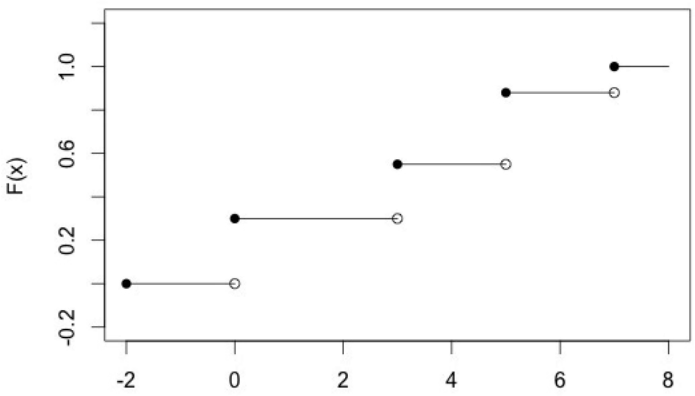
\includegraphics[width=0.75\linewidth]{CdfExamplesReadingProbabilities.png} \end{center}

        \item What is the probability that $X$ is less than $5$?

        $P(x < 5) = 0.55$

        \item What is the probability of $X = 2$?

        $\begin{aligned}[t]
            P(X = 2) & = P(X \le 2) - P(X < 2) \\
                     & = 0.3 - 0.3             \\
                     & = 0
        \end{aligned}$

        Note that $P(X = 2) = 0$ has no changes to CDF on interval of $[0, 3)$. The only outcomes with probability mass are $X = 0$ and $X = 3$. 
    \end{enumerate}
\end{example}

\subsection{Chebyshev's Inequality}

For a given random variable $X$, $\mu_X$ and ${\sigma^2}_X$ are measures of two features of the distribution of $X$: it's `centre' and it's spread. How can we use these two values to better understand the distribution of $X$, especially in the absence of the exact distribution such as the probability mass function (PMF) or the cumulative distribution function (CDF)?

\begin{theorem}[Markov's Inequality]\index{Markov's Inequality}
    Let $X$ be a \bred{non-negative} random variable with mean $E(X)$/ Then, for some constant $\color{red} a > 0$, $$P(X \ge a) \le \frac{E(X)}{a}$$
\end{theorem}

\begin{proof}
    Since $X$ is a non-negative random variable, $\forall x \in X$, $x \ge 0$. 

    Then, $\begin{aligned}[t]
        E(X) & = \sum_{x \in X} x \cdot P(X = x)                                 \\
             & = \sum_{x < a} x \cdot P(X = x) + \sum_{x \ge a} x \cdot P(X = x) \\
             & \ge \sum_{x \ge a} x \cdot P(X = x)                               \\
             & \ge \sum_{x \ge a} a \cdot P(X = x) & \text{since } x \ge a       \\
             & = a \cdot \sum_{x \ge a} P(X = x)                                 \\
             & = a \cdot P(x \ge a)
    \end{aligned}$

    That is, $\begin{aligned}[t]
        E(X)           & \ge a \cdot P(X \ge a) \\
        \frac{E(X)}{a} & \ge P(X \ge a)
    \end{aligned}$
\end{proof}

\begin{theorem}[Chebyshev's Inequality]\index{Chebyshev's Inequality}
    Let $X$ be a random variable with mean (expected value) $\mu$ and finite variance $\sigma^2$. Then for any positive $k$, $$P(|x - \mu| {\color{red}~<~} k\sigma) \ge 1 - \frac{1}{k^2}$$

    Chebyshev's Inequality applies to all discrete distributions with \bred{finite} $E(X)$ and $V(X)$ for the random variable $X$. 
\end{theorem}

\begin{proof}
    $\begin{aligned}[t]
        P(|X - \mu| < k\sigma) & = P((x - \mu)^2 < k^2\sigma^2)         & \text{since RV's are non-nagative and } k > 0 \\
                               & = 1 - (P((x - \mu)^2 \ge k^2\sigma^2))
    \end{aligned}$

    By Markov's Inequality, for a non-negative random variable $X$ and a positive constant $a$, $P(X \ge a) \le \frac{E(x)}{a}$, $a > 0$. Consider $(X - \mu)^2 > 0$ as $x$ and $k^2\sigma^2 > 0$ as $a$ in Markov's Inequality, we have $\begin{aligned}[t]
        P((x - \mu)^2 \ge k^2\sigma^2) \ge \frac{E((x - \mu)^2)}{k^2\sigma^2} & = \frac{\sigma^2}{k^2\sigma^2} \\
                                                                              & = \frac{1}{k^2}
    \end{aligned}$

    That is, $P(|X - \mu| < k\sigma) \ge 1 - \frac{1}{k^2}$. 
\end{proof}

\begin{example}
    Based on past data, the average daily number of tech support requests at a local call centre is 115 with a standard deviation of 10 calls.

    \begin{enumerate}[label=\alph*)]
        \item What can be said about the fraction of days on which the number of calls received is between 100 and 130?
        
        \begin{itemize}
            \item Distribution info: missing 
            \item We are given: $\mu = 115$, $r = 10$
        \end{itemize}

        Let $C$ be the random number of daily calls. 

        $\begin{aligned}[t]
            P(100 \le C \le 130) & = P(-15 \le C - 115 \le 15) \\
                                 & = P(-15 \le C - \mu \le 15) \\
                                 & = P(|C - \mu| \le 15) \\
                                 & = P(|C - \mu| < 16) \\
                                 & = P(|C - \mu| < 1.6\sigma) \\
                                 & \ge 1 - \frac{1}{1.6} = 0.6094
        \end{aligned}$

        $\therefore$ At least $60.94\%$ of the time they will have between 100 to 130 calls a day. 

        \item What number of calls can they expect to receive at least $90\%$ of the time?

        We want to find the number of $\sigma$ that correspond to an interval that has at least $90\%$ chance of occurring. 
        
        $P(|X - \mu| < k\sigma) = 1 - \frac{1}{k^2} = 90\%$

        That is, $\begin{aligned}[t]
            1 - \frac{1}{k^2} & = 0.90        \\
            0.1               & = \frac{1}{k} \\
            k^2               & = 10          \\
            k                 & = \sqrt{10}
        \end{aligned}$

        For all distributions, more than $90\%$ of the outcomes lie within $\sqrt{10} \approx 3.16$ standard derivation of its mean. 

        $(115 - k\sigma, 115 + k\sigma) = (115 - \sqrt{10} \cdot 10, 115 + \sqrt{10} \cdot 10) \approx (83.38, 146.62)$

        $\therefore$ They can expect to receive $[83, 147]$ number of calls at least $90\%$ of the time. 
    \end{enumerate}
\end{example}

\section{Common Discrete Distributions}

\subsection{Binomial Distribution}

\begin{definition}[Bernoulli Trials]\index{Bernoulli Trials}
    A \term{Bernoulli trial} is a random experiment consisting of exactly one trial involving two possible outcomes, often called a \itblue{success} or a \itblue{failure}. Let $X$ be the outcome of a Bernoulli trial where 
    $$\begin{aligned}[t]
        X = 0 & \text{ if the outcome is a failure} \\
        X = 1 & \text{ if the outcome is a success}
    \end{aligned}$$

    We define $p$ to be the probability of \bred{success}, and $q = 1 - p$ to be the probability of \bred{failure}. The \itblue{probability mass function} is then $$f(x) = p^x \cdot (1 - p)^{1 - x}$$
\end{definition}

\begin{example}[Bernoulli Trials]
    Below are some examples of Bernoulli trials. 

    \begin{itemize}
        \item Whether a randomly selected part is defective 
        \item Whether there is an error in a line of code 
        \item Whether a randomly selected individual is taller than 5'7'' 
        \item Whether a switch is in the on or off proposition
        \item Whether your lotto ticket is the winning number
    \end{itemize}
\end{example}

\begin{example}
    Consider a multiple choice quiz $4$ questions. A student selects an answer at random for each question, and each question is a Bernoulli experiment: the student either guesses correctly ($1$) or incorrectly ($0$). The sum of these four Bernoulli experiments will then be the random number of correct answers for a student that completes a similar quiz in this way. Our sample space is: 
    $$\Omega = \left\{ \cmark \cmark \cmark \cmark, \cmark \cmark \cmark \xmark, \cmark \cmark \xmark \cmark, \cmark \xmark \cmark \cmark, \xmark \cmark \cmark \cmark, \cmark \cmark \xmark \xmark, \cmark \xmark \cmark \xmark, \xmark \cmark \cmark \xmark, \xmark \cmark \xmark \cmark, \xmark \xmark \cmark \cmark, \cmark \xmark \xmark \cmark, \right.$$
    $$\left. \xmark \xmark \xmark \cmark, \xmark \xmark \cmark \xmark, \xmark \cmark \xmark \xmark, \cmark \xmark \xmark \xmark, \xmark \xmark \xmark \xmark \right\}$$

    Suppose these MCQs have four options each, and each question only has one correct option. Find the following probabilities. 

    \begin{enumerate}[label=\alph*)]
        \item Guessing each question correctly. 

        $P(\cmark \cmark \cmark \cmark) = \frac{1}{4} \cdot \frac{1}{4} \cdot \frac{1}{4} \cdot \frac{1}{4} = \frac{1}{4^4}$

        \item Guessing each question incorrectly. 

        $P(\xmark \xmark \xmark \xmark) = \frac{3}{4} \cdot \frac{3}{4} \cdot \frac{3}{4} \cdot \frac{3}{4} = \frac{3^4}{4^4}$
        \item Guessing exactly $2$ questions correctly. 

        $P(\cmark \cmark \xmark \xmark) = \frac{1}{4} \cdot \frac{1}{4} \cdot \frac{3}{4} \cdot \frac{3}{4} = \frac{3^2}{4^4}$

        $P(2 \text{ correct}) = _4C_2 \cdot \frac{3^2}{4^4}$
    \end{enumerate}
\end{example}

Often, we are interested in modeling the number of successes among multiple trials instead of the results of a single trial:

\begin{definition}[Binomial Distribution]\index{Binomial Distribution}
    A \term{Binomial experiment} consists of $n$ independent and identical Bernoulli trials. The probability of success, $p$, is fixed for each trial. 

    {~~~}

    Let $X$ be the random variable representing the number of successes among the $n$ trials. Then $X$ can be modeled by the binomial distribution with parameters $n$ and $p$, denoted as $X \sim \mathrm{Bin}(n, p)$. The binomial distribution has probability mass function: $$P(X = x) = \binom{n}{x} \cdot p^x \cdot (1 - p)^{n - x}$$ If $X \sim \mathrm{Bin}(n, p)$, we can show that $E(X) = np$ and $V(X) = np(1 - p)$
\end{definition}

\begin{example}[Binomial Experiments]
    Below are some examples of Binomial experiments. 

    \begin{itemize}
        \item The number of people who tried the dalgona candy challenge following `Squid Game'
        \item The number number of randomly selected students who started playing Animal Crossing in 2020
        \item The number of games won out of $7$ independent games with the same opponent
    \end{itemize}
\end{example}

\begin{example}
    While studying by a window, you find yourself noticing many cars at a nearby intersection that fail to fully come to a stop at the stop sign before passing through the intersection. Based on your months of data, you reliably calculate the probability of drivers failing to do a complete stop to be $70\%$. Assuming the stopping behaviour of each car is independent of all others, find the probability that among $20$ randomly observed cars that...

    \begin{enumerate}[label=\alph*)]
        \item Exactly $5$ will come to a complete stop? 
        
        Let $S$ be the number of cars that stop. 

        $S \sim Bin(n = 20, p = 0.3)$. 

        {~~~}
        
        $\begin{aligned}[t]
            P(S = 5) & = \binom{20}{5} \cdot 0.3^5 \cdot (1 - 0.3)^{20-5}              \\
                     & = \frac{20!}{(20-5)! \cdot 5!} \cdot 0.3^5 \cdot 0.7^{15} \\
                     & \approx 0.1789
        \end{aligned}$

        \item At least $3$ will come to a complete stop?
        
        $\begin{aligned}[t]
            P(S \ge 3)
             & = \sum_{s = 3}^{20} \binom{20}{s} \cdot 0.3^s \cdot (1 - 0.3)^{20-s}                                                                    & \text{(direct)}   \\
             & = 1 - P(S < 3)                                                                                                                          & \text{(indirect)} \\
             & = 1 - P(S \le 2)                                                                                                                                            \\
             & = 1 - \left( \binom{20}{0} \cdot 0.7^{20} + \binom{20}{1} \cdot 0.3^1 \cdot 0.7^{19} + \binom{20}{2} \cdot 0.3^2 \cdot 0.7^{18} \right)                     \\
             & \approx 0.9645
        \end{aligned}$

        \item At most $3$ will come to a complete stop?
        
        $\begin{aligned}[t]
            P(S \le 3) & = P(S = 0) + P(S = 1) + P(S = 2) + P(S = 3)                                                                                                                     \\
                       & = \binom{20}{0} \cdot 0.7^{20} + \binom{20}{1} \cdot 0.3^1 \cdot 0.7^{19} + \binom{20}{2} \cdot 0.3^2 \cdot 0.7^{18} + \binom{20}{3} \cdot 0.3^3 \cdot 0.7^{17} \\
                       & \approx 0.1071
        \end{aligned}$
    \end{enumerate}
\end{example}

\begin{example}
    A  local hospital has several backup generators to support critical technologies in the event of a power outage or failure. Each backup generator is identical in make, and operate independently of others. Suppose each backup generator has a $20\%$ chance of failing when used. How many generators should be installed so that the system has at least a $99.5\%$ probability of functioning in the event of a power outage?

    Let $n$ be the number of generators (a fixed quantity).

    Let $G$ be the number of generators that functions. 

    $G \sim Bin(n, p = 0.8)$. 

    We want to find $n$ such that $P(G \ge 1) \ge 99.5\%$. 

    That is, by the indirect method, we need $\begin{aligned}[t]
        P(G = 0) & \le 0.005 \\
        \binom{n}{0} \cdot 0.2^n \le 0.005 \\
        0.2^n \le 0.005 \\
        n \ge 3.29
    \end{aligned}$

    $\therefore$ At least $4$ generators should be installed. 
\end{example}

\subsection{Poisson Distribution}

Consider modeling of the number of Shiba, $D$, spotted at a nearby park over any 1 day with a probability model. (How is this different from a Binomial model if it still models the number of `successes'?)

\begin{center} 
\includegraphics[width=0.25\linewidth]{doge.jpg} \end{center}

This is \bred{not} a binomial distribution, as trials are \itblue{discrete}, while time is \itblue{continuous}! 

Let's try to formulate this problem so it resembles a Binomial model: first we will arbitrarily divide the 1 day into $n$ equally-sized time interval with the following properties for any one interval:

\begin{itemize}
    \item $P(D = 1) = p$
    \item $P(D = 0) = 1 - p$
    \item $P(D > 1) = 0$ (i.e. the event of Shiba sighting is ``rare'')
\end{itemize}

Let us also assume that each time interval behaves independently, and the average (mean) number of Shiba sightings per day is fixed and denoted by $\lambda$. 

Based on the construction and assumptions, we have $n$ independent trials with equal probabilities of ``success'' $p$. This can be modeled as a binomial distribution where $D \sim Bin(n, p)$, which has an expected values of $E(D) = np$. 

Since the mean number of daily sightings is constant, 

\begin{itemize}
    \item $E(D) = np = \lambda$, and $p = \frac{\lambda}{n}$
    \item The number of time intervals is arbitrarily decided, neither $n$ nor $p$ are known.
    \item In order to ensure daily average $\lambda = np$ remains constant, as $n$ increases, $p$ must decrease so that $np$ remains unchanged
\end{itemize}

We'll get more accurate probabilities of daily sightings in a day if we allow each time interval to shrink to $0$ (not too different from using Riemann sums to approximate area under continuous curves!). Let's see how the binomial PMF behaves as $n \to \infty$ and $p \to 0$.

The resulting function will model the \itblue{probability of $D$ number of Shiba sightings} over a \itblue{continuous period of 1 day}.

Let $D$ be the number of Shiba sighted in ``n'' sub-intervals.

$D \sim Bin(n, p = \frac{\lambda}{n})$. 

$E(D) = np = \lambda$. 

$\begin{aligned}[t]
    P(D = d)
     & = \lim_{n \to \infty} \binom{n}{d} \cdot p^d \cdot (1 - p)^{n - d} \\
     & = \lim_{n \to \infty} \frac{n!}{(n - d)! \cdot d!} \cdot \left( \frac{\lambda}{n} \right)^d \cdot \left( 1 - \frac{\lambda}{n} \right)^{n - d} \\
     & = \frac{\lambda^d}{d!} \lim_{n \to \infty} \frac{n(n-1)(n-2)\cdots(n-d+1)\cancel{(n-d)!}}{\cancel{(n-d)!}} \cdot \frac{1}{n^d} \left( 1 - \frac{\lambda}{n} \right)^{n-d} \\
     & = \frac{\lambda^d}{d!} \lim_{n \to \infty} \frac{n}{n} \times \frac{n-1}{n} \times \frac{n-2}{n} \times \cdots \times \frac{n-d+1}{n} \cdot \left( 1 - \frac{\lambda}{n} \right)^{n-d} \\
     & = \frac{\lambda^d}{d!} \lim_{n \to \infty} \left( 1 \right) \left( 1 - \frac{1}{n} \right) \left( 1 - \frac{2}{n} \right) \cdots \left(1 - \frac{d-1}{n} \right) \left( 1 - \frac{\lambda}{n} \right)^{n-d} \\
     & = \frac{\lambda^d}{d!} \lim_{n \to \infty} \left( 1 - \frac{\lambda}{n} \right)^{n-d} \\
     & = \frac{\lambda^d}{d!} \lim_{n \to \infty} \left( 1 - \frac{\lambda}{n} \right)^n \cancelto{1}{\left( 1 - \frac{\lambda}{n} \right)^{-d}} \\
     & = \frac{\lambda^d}{d!}  \cdot e^{-\lambda} \qquad \text{as } \lim_{n \to \infty} \left( 1 - \frac{\lambda}{n} \right)^n = e^{-\lambda} \\
     & = \frac{\lambda^d e^{-\lambda}}{d!}
\end{aligned}$

\begin{definition}[Poisson Distribution]\index{Poisson Distribution}
    A discrete random variable $X$ denoting the number of (sometimes rare) events of interest in an interval, with the mean number of occurrences per unit interval denoted by $\lambda$, is \term{Poisson Distributed} if it has the probability mass function $$P(X = x) = \frac{\lambda^x e^{-\lambda}}{x!}$$

    $X$ has expectation $E(X) = \lambda$ and variance $V(X) = \lambda$. 
\end{definition}

Note that $\lambda$ is also called the \term{rare parameter} as it describes the average \itblue{rate of occurrance} of the event. $\lambda$ should always be adjusted for the time interval being considered. 

Poisson distribution is appropriate for discrete random variables that count the number of occurrences in a \bred{continuous interval} where

\begin{itemize}
    \item No more than one occurrence can occur simultaneously 
    \item Non-overlapping intervals have occurrences that behave independently 
    \item Expected number of occurrences in each fixed time interval is constant
\end{itemize}

As suggested in the construction of the Poisson distribution, this distribution can be used to approximate binomial probabilities where $n$ is large and $p$ is small. The approximation improves as $n$ increases and/or $p$ decreases. The advantage here is that Poisson distribution can be easier to compute since it doesn't involve the $\binom{n}{x}$ factor in its PMF. 

What does a Poisson distribution look like? Generally unimodal and right-skewed, there is greater likelihood in observing values near but less than the mean $\lambda = 4$.

\begin{center} 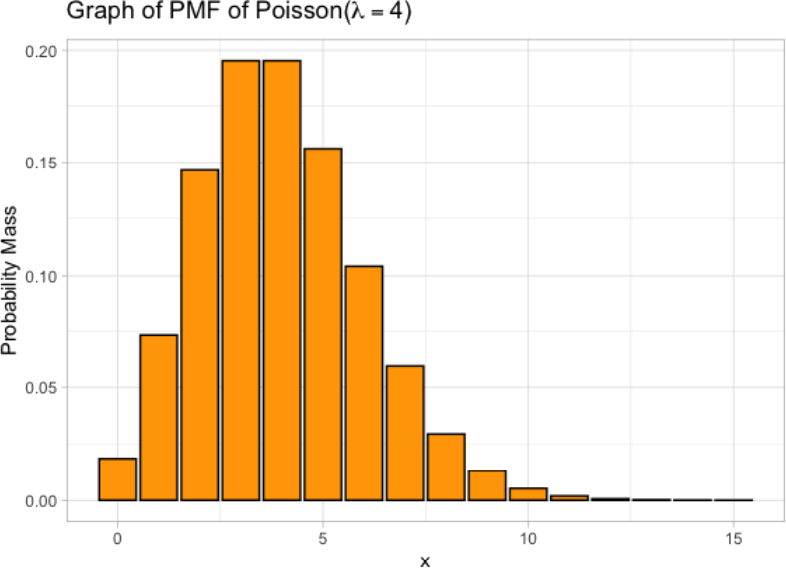
\includegraphics[width=0.75\linewidth]{PoissonDistributionPlot.png} \end{center}

\begin{example}
    An area of a forest as on average $6$ trees per $100$ m\textsuperscript{2}. 

    \begin{enumerate}[label=\alph*)]
        \item Do the assumptions for a Poisson model seem appropriate for modeling tree distribution in a forest
        
        \begin{itemize}
            \item Two simulations trees (two trees occupying the same spot) is $0$
            \item Could reasonably assume that the number of trees per area is independent
        \end{itemize}

        \item What is the probability of having at least $1$ tree in a $100$ m\textsuperscript{2} area? 
        
        Let $T$ be the number of trees per $100$ m\textsuperscript{2}. 

        $T \sim Pois(\lambda = 6)$. 

        Using the indirect method, $\begin{aligned}[t]
            P(T \ge 1) & = 1 - P(T = 0)              \\
                       & = 1 - \frac{6^0 e^{-6}}{0!} \\
                       & \approx 0.9975
        \end{aligned}$

        $\therefore$ There is $99.75\%$ change of having at least $1$ tree in a $100$ m\textsuperscript{2} area. 
    \end{enumerate}
\end{example}

\begin{example}
    The number of car repairs $R$ that arrive at a mechanic can be well modeled by a Poisson random variable with a mean of $3t$, where $t$ denotes the time in hours of operating hours. The average profit per repair is given by $Y = 85R^2 - 60t$. Assuming that vehicle arrival occurs independently,

    \begin{enumerate}[label=\alph*)]
        \item What is the probability that in a $10$ hour workday, they will service between $28$ to $31$ cars? 

        We can reasonably model $R \sim Pois(\lambda = 3 \cdot 10 = 30)$. 

        Then, $\begin{aligned}[t]
            P(28 \le R \le 31)
             & = \sum_{r=28}^{31} P(R = r)                                                                                             \\
             & = \frac{30^{28} e^{-30}}{28!} + \frac{30^{29} e^{-30}}{29!} + \frac{30^{30} e^{-30}}{30!} + \frac{30^{31} e^{-30}}{31!} \\
             & \approx 0.2858
        \end{aligned}$

        $\therefore$ $28.58\%$ of the time they will service between $28$ to $31$ cars. 

        \item What is the corresponding profit earned for the cars serviced in a)? 

        $Y = 85R^2 - 60 \cdot 10 = 86R^2 - 600$ with $R \in [28, 31]$.

        That is, $y \in [85 \cdot 28^2 - 600, 85 \cdot 31^2 - 600] = [66040, 81085]$

        $\therefore$ They are expected to earn from $\$66,040$ to $\$81,085$. 

        \item What is the expected profit for a typical $8$ hour workday?

        $R \sim Pois(\lambda = 3 \cdot 8 = 24)$
        
        $\begin{aligned}[t]
            E(Y) & = E(85R^2 - 60 \cdot 8) \\
                 & = E(85R^2 - 480) \\
                 & = 85 E(R^2) - 480 \\
        \end{aligned}$

        Since $V(R) = E(R^2) - E(R)^2$, $E(R^2) = V(R) + E(R)^2 = \lambda + \lambda^2 = 24 + 24^2$. 

        Then, $\begin{aligned}[t]
            E(Y) & = 85 (24 + 24^2) - 480 \\
                 & = \$50,520
        \end{aligned}$

        $\therefore$ The expected profit for a typcail $8$ hour workday is $\$50,520$. 

        \item Suppose that you know that in an 8 hour workday, $E(R^4) = 416,472$. Determine the variance in profit. Can you determine what interval of profits they can expect to earn with at least $75\%$ probability?

        $R \sim Pois(24)$. 

        $E(Y) = 50,520$

        $\begin{aligned}[t]
            V(Y) & = V(85R^2 - 480) = 85^2 \cdot V(R^2)  \\
                 & = 85^2 \cdot (E((R^2)^2) - E(R^2)^2)  \\
                 & = 85^2 \cdot (416,472 - (24 + 24^2)^2) \\
                 & = \$^2 408,010,200
        \end{aligned}$

        {~~~}

        $\sigma_Y = \sqrt{V(Y)} \approx \$20,199.26$

        By Chebyshev, $P(|Y - \mu_Y| < k\sigma_Y) \ge 1 - \frac{1}{k^2}$, and we want $1 - \frac{1}{k^2} = \frac{3}{4}$. That is, $k = 2$. 

        $y \in (50520 - 2(20199.26), 50520 + 2(20199.26)) = (10121.48, 90918.52)$

        $\therefore$ They are expected to earn within $(10121.48, 90918.52)$ with at least $75\%$ probability. 
    \end{enumerate}
\end{example}

%----------------------------------------------------------------------------------------
%	BIBLIOGRAPHY
%----------------------------------------------------------------------------------------

%\chapter*{Bibliography}
%\addcontentsline{toc}{chapter}{\textcolor{ocre}{Bibliography}}
%\section*{Books}
%\addcontentsline{toc}{section}{Books}
%\printbibliography[heading=bibempty,type=book]
%\section*{Articles}
%\addcontentsline{toc}{section}{Articles}
%\printbibliography[heading=bibempty,type=article]

%----------------------------------------------------------------------------------------
%	INDEX
%----------------------------------------------------------------------------------------

\cleardoublepage
\phantomsection
\setlength{\columnsep}{0.75cm}
\addcontentsline{toc}{chapter}{\textcolor{ocre}{Index}}
\printindex

%----------------------------------------------------------------------------------------

\end{document}
